\documentclass[5p,times,twocolumn]{elsarticle}
\usepackage{amssymb}
\usepackage[utf8]{inputenc}
\usepackage[T1]{fontenc}
\usepackage{textcomp}
\usepackage{xcolor}
\usepackage{graphicx}
\usepackage{seqsplit}
\usepackage{url}
\usepackage[hidelinks]{hyperref}
\usepackage{placeins}
\journal{Biomaterials and Biosystems}

\begin{document}

\begin{frontmatter}

\title{Cross-Material Design Strategies in Hydroxyapatite-, Chitosan-, and Polycaprolactone-Based Scaffolds: A Systematic Review of Biological Performance and Evidence Quality}

\author[label1]{Ethan Nicolás García San Andrés}
\author[label2]{Juan Carlos García Plúa}

\address[label1]{Universidad Politécnica Salesiana, Guayaquil, Ecuador}
\address[label2]{Universidad de Guayaquil, Guayaquil, Ecuador}

\begin{abstract}
Hydroxyapatite, chitosan, and polycaprolactone (PCL) are among the most widely studied biomaterials for tissue engineering scaffolds, yet evidence on their design strategies and biological performance remains fragmented. This systematic review (PRISMA 2020) searched Scopus and Web of Science for articles from 2023 onward; of 564 records identified, 78 studies meeting pre-specified eligibility criteria were included. PCL was the most frequent principal material (30/78 studies), followed by chitosan (22/78) and hydroxyapatite (17/78). Biocompatibility outcomes were reported across the specific formulations tested, with hydroxyapatite associated with osteogenic outcomes, chitosan with cell adhesion and antibacterial activity, and PCL with mechanical stability. A concentration-dependent response pattern was examined across 19 candidate studies; five did not, on closer inspection, reflect a chemical concentration series, and of the remaining 14, only 7 show a genuine non-monotonic (interior-optimum) response, while the others reflect a boundary effect, a composition/formulation comparison, or a cross-outcome trade-off, so this observation is presented as a qualitative, per-study-categorized finding rather than a uniform pattern or a validated design rule. A complementary BioBERT-based text-mining analysis of the same corpus did not reproduce a clean bioactivity-versus-mechanical-support split between these two materials: hydroxyapatite was the most conceptually central material in composition-related text and the one most directly linked to bone, whereas PCL was, somewhat counterintuitively, the most central node in fabrication-strategy, engineering-property, and biological-function text alike, with hydroxyapatite and PCL comparably central to each other only in tissue-application text, where bone was the dominant node overall. These findings reflect predominantly in vitro, modification-specific evidence --- because all 30 PCL studies applied at least one modification strategy, conclusions regarding PCL do not extend to the unmodified polymer. Overall, biomaterial selection should be guided by tissue-specific functional roles and by the maturity of the underlying evidence rather than a universal hierarchy.
\end{abstract}

\begin{keyword}
tissue engineering scaffold \sep hydroxyapatite \sep chitosan \sep polycaprolactone \sep biocompatibility \sep scaffold modification \sep systematic review \sep PRISMA
\end{keyword}

\end{frontmatter}


\section{Introduction}

Tissue engineering scaffolds are three-dimensional, typically porous, structures designed to support cell adhesion, proliferation, and differentiation while guiding the regeneration of damaged or lost tissue. Among the broad range of materials explored for this purpose, hydroxyapatite, chitosan, and polycaprolactone (PCL) are consistently among the most frequently studied representatives of their respective material classes --- a synthetic calcium-phosphate ceramic, a natural polysaccharide, and a synthetic biodegradable polyester, respectively \cite{ref79}.

Hydroxyapatite is compositionally similar to the mineral phase of native bone and is widely used to confer osteoconductive and osteoinductive properties to a scaffold \cite{ref80}. Chitosan, derived from chitin, offers intrinsic biocompatibility, biodegradability, and antibacterial activity, and is frequently combined with other materials to improve cell adhesion \cite{ref81}. PCL is valued for its slow, controllable degradation and favorable mechanical processability, including compatibility with 3D printing and electrospinning, though its intrinsic bioactivity is comparatively limited \cite{ref82}.

Despite the individual maturity of the literature on each of these three materials, the specific design strategies used to modify them --- nanoparticle incorporation, surface functionalization, crosslinking, growth factor loading, and structural design, among others --- are reported using highly heterogeneous experimental designs, outcome measures, and reporting standards, making direct comparison across studies difficult without a systematic synthesis.

This review addresses a central question: which design strategies applied to hydroxyapatite, chitosan, and PCL scaffolds have been reported to improve biocompatibility and biological performance in tissue engineering, and how do these reported effects compare across materials? This question is addressed through three sub-questions:

Q1: Among hydroxyapatite, chitosan, and PCL scaffolds, which biocompatibility-related outcomes (e.g., cell viability, adhesion, osteogenic activity, antibacterial activity) are most frequently reported with each material, based on the reported evidence?

Q2: Which modification strategies (crosslinking, surface functionalization, nanoparticle incorporation, growth factor loading) have been applied to hydroxyapatite, chitosan, and PCL scaffolds, and what biological effects are reported for each?

Q3: What does entity co-occurrence network analysis reveal about the relative conceptual centrality of hydroxyapatite and PCL across five content axes (material, fabrication, engineering property, biological function, and tissue application), and what bridge concepts connect otherwise disconnected thematic sub-domains? (addressed in Section~\ref{sec:q3})

Hydroxyapatite, chitosan, and PCL scaffolds have each already been the subject of recent single-material reviews \cite{ref80,ref81,ref82}; this review's novelty is a recent cross-material synthesis spanning all three within one evidence base, detailed further in the Discussion.

\section{Methodology}

\subsection{Protocol and Reporting Standard}

This systematic review was conducted following the PRISMA 2020 (Preferred Reporting Items for Systematic Reviews and Meta-Analyses) guidelines (Page et al., 2021). The review addresses a central research question and two evidence-based sub-questions, with a third, data-driven sub-question (BioBERT-based topic modeling and biomedical entity co-occurrence network analysis of the extracted corpus) addressed separately in Section~\ref{sec:q3}, using the data extracted through the process described below. This review was not prospectively registered (e.g., PROSPERO) and no separate protocol was published beforehand; this is disclosed for PRISMA 2020 compliance and treated as a limitation in Section~\ref{sec:discussion}. Given the heterogeneity in designs, outcomes, and reporting formats across included studies (Section~1), a narrative, structured synthesis was adopted instead of a meta-analysis; no pooled effect size was calculated for any outcome.

\subsection{Focus Materials and Rationale}

The review was scoped to three biomaterials --- hydroxyapatite, chitosan, and polycaprolactone (PCL) --- selected as the most frequently cited representatives of their material categories (ceramic, natural polymer, synthetic polymer) within the tissue engineering scaffold literature. Broader categorical searches (e.g., ``natural'', ``synthetic'', ``ceramic'') were piloted but discarded for producing results too heterogeneous for consistent cross-study comparison.

\subsection{Search Strategy}

Two bibliographic databases were searched: Scopus and Web of Science (Core Collection). Searches were last executed in August 2026. Searches were restricted to original research articles (document type ``article''), published in English, from 2023 onward (PUBYEAR $>$ 2022); this recent four-year window was chosen to capture the most recent generation of scaffold design strategies while keeping the corpus focused enough for detailed full-text extraction, and is consistent with the field's rapid rate of methodological change. The base Boolean string combined a tissue-engineering scaffold term, a materials term, and a question-specific term block, adapted to the syntax of each database:

\begin{quote}
\textit{TITLE-ABS-KEY(``tissue engineering scaffold*'') AND TITLE-ABS-KEY(hydroxyapatite OR chitosan OR polycaprolactone OR PCL) AND TITLE-ABS-KEY([question-specific block]) AND (LIMIT-TO(DOCTYPE,``ar'')) AND (LIMIT-TO(LANGUAGE,``English''))}
\end{quote}

Two question-specific blocks were used, corresponding to the review's two evidence-based sub-questions:
\begin{itemize}
\item Q1 block (biocompatibility outcomes): biocompatib* OR cytocompatib* OR ``cell viability'' OR cytotox* OR ``cell proliferation'' OR ``cell adhesion''
\item Q2 block (modification strategies): crosslink* OR ``surface modification'' OR functionali?ation OR ``growth factor*'' OR nanoparticle* OR coating OR ``drug loading''
\end{itemize}

\begin{table}[h]
\caption{Records identified per database and sub-question.}
\label{tab:search}
\small
\begin{tabular}{p{1.6cm}p{1.2cm}p{3cm}p{1.3cm}}
\hline
\textbf{Database} & \textbf{Sub-Q} & \textbf{Search block added} & \textbf{n} \\
\hline
Scopus & Q1 & biocompatib* OR cytocompatib* OR ``cell viability'' & 188 \\
Scopus & Q2 & crosslink* OR ``surface modification'' OR nanoparticle* & 105 \\
Web of Science & Q1 & (same block, adapted syntax) & 169 \\
Web of Science & Q2 & (same block, adapted syntax) & 102 \\
\hline
\textbf{Total} & & & \textbf{564} \\
\hline
\end{tabular}
\end{table}

A total of 564 records were identified across the four searches (188 + 105 in Scopus; 169 + 102 in Web of Science).

\subsection{Eligibility Criteria}
\label{sec:eligibility}

Eligibility was assessed in two sequential stages.

\textbf{Stage 1 --- Thematic screening (title and abstract).} Inclusion criteria: (i)~original research article (reviews excluded); (ii)~at least one of the three focus materials present as a principal component of the study, not merely as a minor additive or comparator; (iii)~English language; (iv)~document type ``article'' (conference papers and book chapters excluded). Exclusion criteria: review articles; studies limited to purely physicochemical characterization without a biological/cellular component; studies in which the focus material served only as a minor comparator or additive; studies with an anticancer cytotoxicity objective (i.e., aiming to kill cells, the inverse of a biocompatibility objective); duplicate records.

\textbf{Stage 2 --- Evidence-based screening (full text).} Eligibility at Stage 2 required, first, that the full text be retrievable through the authors' institutional access, interlibrary loan, or lawful open-access channels within the review period (through August 2026); records for which the full text could not be retrieved were excluded at this stage on that basis alone. For records meeting this access criterion, a record was retained (PASS) if it reported at least one of the following: (i)~an explicit quantitative biocompatibility or biological-performance value (percentage, figure with standard deviation, or statistical result); or (ii)~an explicit, clear comparison between experimental groups or formulations with a differentiated biological outcome, even in the absence of an exact percentage. A record was excluded (FAIL) if it reported only an isolated qualitative statement (e.g., ``good/excellent biocompatibility'') without a supporting quantitative value or comparison, or if the full text could not be retrieved.

Of the 564 records identified, 69 were removed as duplicates, and of the resulting 495 unique records, 371 were excluded at Stage 1 based on title and abstract review, primarily for not meeting the material-relevance criterion (focus material not present as a principal component) or for being review articles, conference papers, or non-English publications.

\subsection{Study Selection Process}

Study selection followed the standard PRISMA identification--screening--eligibility--inclusion sequence. Search exports from both databases were first consolidated and deduplicated, prior to Stage 1 (title/abstract) screening. Deduplication was performed using the Digital Object Identifier (DOI) as the matching key, normalized to lowercase with whitespace trimmed, in three sequential passes: (1)~within each database, across the Q1 and Q2 search exports; (2)~a manual cross-reference pass in which 13 additional Scopus records were identified as redundant and removed; and (3)~a final cross-database pass between the Scopus and Web of Science sets, in which Scopus records were retained preferentially in the event of a match. This process reduced the 564 identified records to 495 unique records, which were then screened against the Stage 1 (title/abstract) eligibility criteria (Section~2.4), yielding 124 records eligible for full-text assessment.

Full-text retrieval was attempted for all 124 records remaining after Stage 1 screening. Of these, 37 could not be retrieved through institutional access, interlibrary loan, or lawful open-access channels within the review period, and were excluded on that access-based criterion alone (Section~2.4) without content-based assessment. The remaining 87 records were assessed for eligibility against the content-based criteria described above by the first author; 9 were excluded, with reasons summarized in Table~\ref{tab:excl}. The remaining 78 records were retained for the final synthesis. Screening was performed by a single reviewer rather than independently by two, a less stringent design than full dual independent screening; this is acknowledged as a limitation in Section~2.7.

\begin{figure*}[t]
\centering
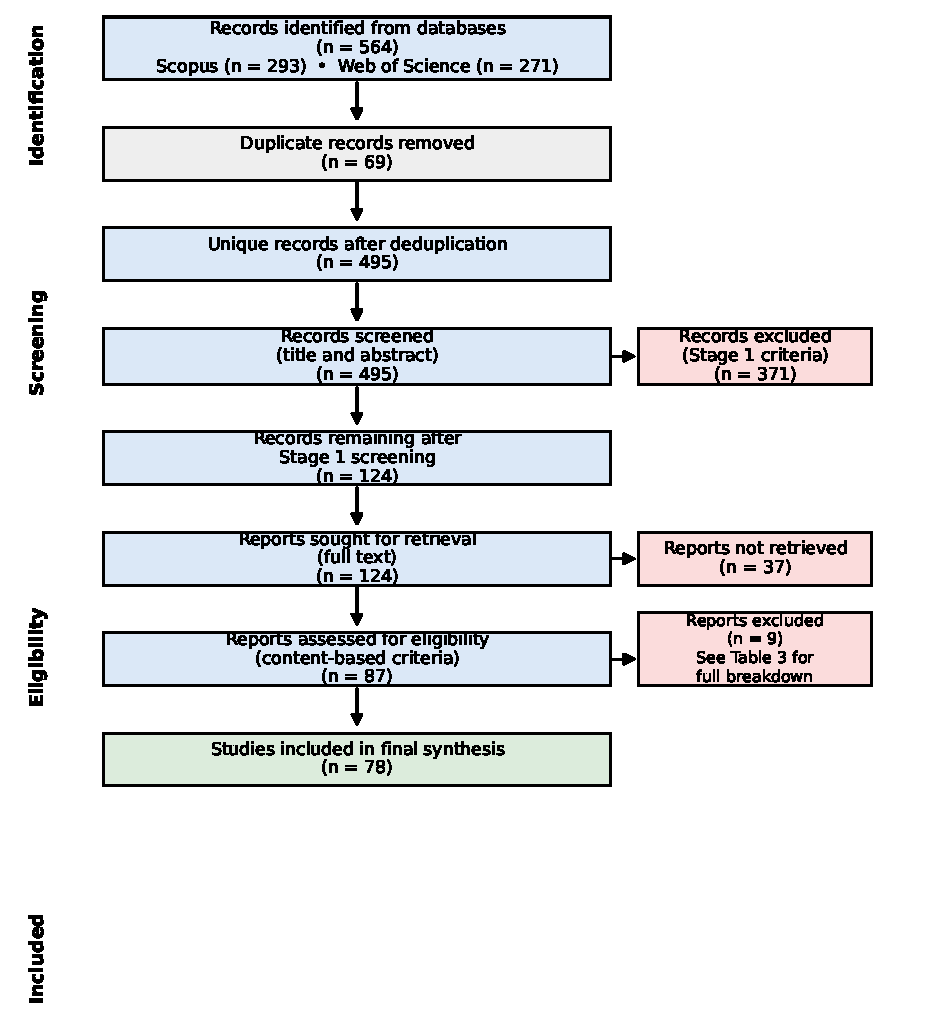
\includegraphics[height=0.5\textheight,keepaspectratio]{figures/figura1_prisma.pdf}
\caption{PRISMA 2020 flow diagram summarizing the identification, screening, eligibility, and inclusion stages of this systematic review.}
\label{fig:prisma}
\end{figure*}

\begin{table}[h]
\caption{PRISMA flow summary.}
\label{tab:prisma}
\small
\begin{tabular}{p{5cm}p{1cm}}
\hline
\textbf{PRISMA stage} & \textbf{n} \\
\hline
Records identified (Scopus + WoS) & 564 \\
Duplicate records removed & 69 \\
Unique records after deduplication & 495 \\
After Stage 1 (title/abstract) screening & 124 \\
Reports sought for retrieval (full text) & 124 \\
Reports not retrieved & 37 \\
Reports assessed for eligibility (full text) & 87 \\
Excluded after assessment, with reasons (Table~\ref{tab:excl}) & 9 \\
\hline
\textbf{Included in final synthesis} & \textbf{78} \\
\hline
\end{tabular}
\end{table}

\begin{table}[h]
\caption{Reasons for exclusion after full-text assessment, among the 87 records whose full text was retrieved and assessed for eligibility (n = 9 excluded). This is distinct from the 37 records excluded earlier solely because their full text could not be retrieved (Table~\ref{tab:prisma}), which were never assessed against these content-based criteria.}
\label{tab:excl}
\small
\begin{tabular}{p{1.6cm}p{1.7cm}p{3.7cm}}
\hline
\textbf{Records} & \textbf{Criterion} & \textbf{Specific reason} \\
\hline
5 records & Stage 1 & HA, chitosan, or PCL used only as comparator/reference, not principal component (e.g., PLGA-, Ti-, PLA-, TCP-, or PEOT-PBT-based scaffolds) \\
1 record & Stage 1 / scope & Purely computational modelling study (Bayesian neural network), no original experimental biological data \\
1 record & Stage 1 & Principal material was not HA, chitosan, or PCL; chitosan appeared only incidentally as a buffer component \\
2 records & Stage 2 & Reported only an isolated qualitative statement (e.g., ``adequate viability, no toxicity'') without supporting quantitative value or comparison \\
\hline
\end{tabular}
\end{table}

\subsection{Data Extraction}

For each of the 78 included studies, data were extracted using a standardized template covering: study identifier; title, authors, and year; focus material(s); modification strategy; assay type (in vitro/in vivo, cell line or animal model); the specific quantitative outcome reported, with units; and the sub-question(s) addressed. This structured extraction dataset supports the quantitative synthesis in Sections~\ref{sec:results}--\ref{sec:discussion} (Q1, Q2); the complementary analysis in Section~\ref{sec:q3} (Q3) instead uses the full text of the included studies as its input corpus.

\subsection{Limitations of the Search Strategy}

This review searched two bibliographic databases (Scopus and Web of Science). While this dual-database approach improves coverage relative to a single-source search, it remains a narrower search than reviews additionally incorporating PubMed/MEDLINE or Embase, which index somewhat different subsets of the biomedical literature. This is acknowledged as a limitation; future work could extend the search to a third database to further improve recall.

\section{Results}
\label{sec:results}

Consistent with this review's central aim, the results below are organized around the design-to-outcome chain requested for this synthesis: which design variable was manipulated (Section~\ref{sec:strategies}), what physicochemical or structural consequence this produced, what biological or cellular response followed (Section~\ref{sec:biocompat}), and at what evidence tier --- in vitro only versus in vivo-validated --- this response was demonstrated. Section~\ref{sec:materials} first summarizes the distribution of the three focus materials across the 78 included studies; Section~\ref{sec:pattern} then reports a cross-cutting concentration-dependent pattern that recurs across this chain in multiple materially unrelated systems.

\subsection{Study Selection}

The search and screening process is summarized in the PRISMA flow diagram (Table~\ref{tab:prisma}). Of 564 records identified across Scopus and Web of Science, 78 studies met both the thematic (Stage 1) and evidence-based (Stage 2) eligibility criteria and were retained for data synthesis.

\subsection{Distribution of Focus Materials Across Included Studies}
\label{sec:materials}

Hydroxyapatite, chitosan, and PCL were represented across the 78 included studies, with PCL as the single most frequent principal material, followed by chitosan and hydroxyapatite; a smaller subset of studies combined two of the three focus materials within the same scaffold system (Table~\ref{tab:materials}). A structured Material $\times$ Strategy $\times$ Tissue-Application $\times$ Outcome $\times$ Evidence-Type matrix for all 78 studies, cross-referencing focus material, modification strategy, target tissue application, outcome summary, and the type of quantitative or comparative evidence reported, is provided as Supplementary Table~S3.

\begin{table}[h]
\caption{Distribution of principal materials.}
\label{tab:materials}
\small
\begin{tabular}{p{4.5cm}p{1.5cm}}
\hline
\textbf{Principal material} & \textbf{n = 78} \\
\hline
Polycaprolactone (PCL) & 30 \\
Chitosan & 22 \\
Hydroxyapatite (HA) & 17 \\
Combined (PCL+HA, PCL+CS, CS+HA) & 9 \\
\hline
\end{tabular}
\end{table}

\subsection{Modification Strategies and Their Reported Effects (Sub-Question 2)}
\label{sec:strategies}

This section addresses the first link in the design-to-outcome chain introduced above: which design variable was manipulated, and what immediate physicochemical or structural consequence it produced, before that consequence is connected to a biological response in Section~\ref{sec:biocompat}.

\textbf{Nanoparticle incorporation.} Fourteen studies incorporated inorganic or organic nanoparticles into a chitosan-, PCL-, or HA-based matrix \cite{ref4,ref6,ref8,ref9,ref12,ref19,ref22,ref24,ref27,ref31,ref68,ref71,ref72,ref74}. A representative dose-dependent pattern was observed for zinc oxide in chitosan matrices, where 3 wt\% ZnO produced optimal biocompatibility and bioactivity in both in vitro and in vivo assessments \cite{ref19}. A hydroxyapatite-based system comparing CuO- and ZnO-doped nanocomposites reported markedly higher Vickers hardness and substantially higher cell viability for the CuO-doped formulation relative to the ZnO-doped one at equivalent concentrations \cite{ref22}, indicating that the identity of the dopant, not only its presence, materially affects biological performance.

\textbf{Growth factor loading.} Nine studies loaded a specific growth factor or bioactive peptide (BMP-2, BMP-7, IGF-1, bFGF, NGF, VEGF-mimetic peptide, or a platelet-rich fibrin derivative) onto a chitosan or PCL carrier \cite{ref7,ref8,ref10,ref25,ref42,ref72,ref75,ref76,ref77}. Reported outcomes included sustained release profiles extending from 72~h to 28~days; where an antibacterial agent was co-delivered alongside a growth factor, the growth factor counteracted the antiproliferative side effect of the antibacterial agent on host cells while preserving antibacterial efficacy (inhibition zone of 21.16~mm against \textit{S. aureus} with 93--96\% cumulative release of both agents over 28~days) \cite{ref25}.

\textbf{Surface functionalization and coatings.} Thirteen studies applied a post-fabrication surface treatment --- aminolysis, plasma treatment, polydopamine coating, or a gelatin overcoat --- to a PCL or PCL/HA scaffold \cite{ref18,ref25,ref26,ref46,ref53,ref54,ref55,ref60,ref68,ref72,ref73,ref76,ref77}. A gelatin coating applied after aminolysis increased mechanical strength by approximately 20\% and Young's modulus by more than 50\%, alongside more than a twofold increase in osteogenic gene expression, relative to the uncoated scaffold \cite{ref18}. Conversely, a polydopamine coating intended to improve cell adhesion on PCL nanoneedle arrays inadvertently reduced the multipotency of seeded mesenchymal stem cells by disrupting cell--cell contact \cite{ref60}, illustrating that surface modifications aimed at one outcome can trade off against another.

\textbf{Crosslinking.} Seven studies manipulated crosslinking density or chemistry as the primary modification strategy \cite{ref1,ref5,ref12,ref16,ref18,ref54,ref61}. Reported effects included tunable compressive and tensile moduli spanning more than three orders of magnitude as a function of hydrogel concentration \cite{ref51}, and improved anisotropic mechanical behavior approaching that of native cortical bone when crosslinking was combined with a directional fabrication pattern \cite{ref1}.

\textbf{Structural and fabrication design.} Eleven studies modified scaffold performance primarily through architectural design --- pore size, printing pattern, or fiber alignment --- rather than through the addition of a bioactive agent \cite{ref1,ref11,ref16,ref17,ref32,ref39,ref40,ref45,ref62,ref63,ref71}. Reported pore-size ranges associated with favorable cell infiltration spanned approximately 10 to 590~$\mu$m depending on the target tissue, and one 3D-printing study reduced print-error rates by up to 85\% through ink and process optimization alone \cite{ref39}.

\textbf{Antibiotic/drug loading.} Four studies loaded a small-molecule drug or a photosensitizer alongside the structural material \cite{ref25,ref31,ref33,ref72}, generally to add antibacterial or antimicrobial functionality; cumulative drug release of 93--95\% within 7--28~days was reported across these systems.

A smaller number of additional studies in the extraction dataset combined structural, drug-delivery, or stimuli-responsive design elements not captured by a single category above, including self-healing or shape-memory matrices and controlled-release fiber or fibrous-scaffold systems \cite{ref3,ref35,ref78}.

\subsection{Biocompatibility Outcomes by Material (Sub-Question 1)}
\label{sec:biocompat}

Building on the design variables and physicochemical consequences described in Section~\ref{sec:strategies}, this section reports the resulting biological response by material, together with the evidence tier --- in vitro only versus in vivo-validated --- at which each response was demonstrated.

Across the 78 included studies, all three focus materials were reported as biocompatible in the specific formulations and systems in which they were studied, with modification strategies serving primarily to enhance --- rather than establish --- cell viability, adhesion, proliferation, and differentiation. It should be noted that for PCL in particular, all 30 included studies applied at least one modification strategy; consequently, the biocompatibility of unmodified PCL specifically cannot be established from this evidence base, and the reported biocompatibility reflects PCL-based systems as studied rather than the base polymer in isolation.

Hydroxyapatite-based studies most frequently reported osteogenic outcomes (alkaline phosphatase activity, calcium deposition, upregulation of RUNX2/OCN/OPN), consistent with hydroxyapatite's compositional similarity to native bone mineral. Several studies explored non-synthetic hydroxyapatite sources --- fish bone \cite{ref70} and discarded teeth \cite{ref32} --- reporting comparable or superior bioactivity and degradation behavior relative to commercial hydroxyapatite. Other hydroxyapatite-based systems explored ion- or metal-oxide-doped formulations, composite 3D-printing inks, and combination with bioactive glass or polymeric carriers to further tune bioactivity, degradation, and mechanical performance \cite{ref2,ref41,ref48,ref52,ref66,ref69}.

Chitosan-based studies most frequently reported favorable cell adhesion and antibacterial activity attributable to chitosan's inherent cationic character, with one study demonstrating that mechanical and degradation properties could be tuned without any chemical crosslinking agent, solely through control of hydrogel water content \cite{ref51}. Additional chitosan-based systems combined chitosan with nanosilver, other polysaccharides, or ceramic fillers to target wound-healing, cartilage, and bone-defect applications \cite{ref13,ref14,ref20,ref23,ref56,ref58}.

PCL-based studies most frequently reported favorable long-term structural stability and mechanical robustness, consistent with PCL's slow degradation kinetics, but comparatively lower intrinsic bioactivity than hydroxyapatite or chitosan when used without a bioactive additive. Additional PCL-based systems in the extraction dataset incorporated magnetic, piezoelectric, or metal-nanoparticle functionalization, together with dynamic-culture and vascular- or cancer-targeted scaffold designs \cite{ref21,ref29,ref38,ref47,ref49,ref64}. Two of these (\cite{ref47,ref64}) mention a cancer-related application without being excluded under this review's anticancer-cytotoxicity criterion (Section~\ref{sec:eligibility}): \cite{ref64} evaluates photothermal ablation of bone-cancer cells as one of two paired endpoints alongside genuine bone-regeneration outcomes in healthy osteoblast-like cells, and \cite{ref47} targets magnetic nanoparticle delivery with no cytotoxic endpoint at all; neither has cell-killing as its stated objective, which is what the exclusion criterion targets. Consistent with this, all 30 PCL-based studies included in this review paired PCL with at least one modification strategy rather than reporting on unmodified PCL alone. Because all PCL studies included in the present corpus involved at least one modification, the findings synthesized here apply to modified or composite PCL-based scaffold systems and should not be interpreted as evidence for unmodified PCL; the statement of comparatively lower intrinsic bioactivity is therefore informed by the broader materials-science literature on PCL rather than by an internal experimental contrast within this review's 78 included studies.

Across the full evidence base, the maturity of this evidence also varies systematically by evidence tier and by tissue application. Of the 78 included studies, 27 reported in vivo or chorioallantoic-membrane (CAM) outcomes in addition to in vitro data and were formally risk-of-bias assessed with SYRCLE (Supplementary Table~S5), while 51 relied on in vitro evidence alone; claims about clinical-scale performance are consequently better supported for the in-vivo-validated subset than for the corpus as a whole. The evidence base was also substantially weighted toward bone-related applications (40/78 studies), whereas soft-tissue and specialized applications such as tendon (1/78), cartilage (4/78), skin/wound (5/78), neural tissue (5/78), and bladder (1/78) were represented by comparatively few studies, alongside a vascular cluster (2/78) and 20/78 studies with no specific tissue target; the material--strategy relationships reported above should therefore not be assumed to generalize across tissue types, particularly where evidence remains sparse. This primary-tissue count treats each study as targeting one tissue; two studies were additionally identified, on a full re-screen of the extraction text, as explicitly targeting a second, distinct tissue or application (a dual-zone bone/nerve scaffold and a combined bone-cancer-therapy/bone-regeneration scaffold) and are flagged with a second label in Supplementary Table~S3 (\texttt{Tissue\_Application\_Secondary}) rather than folded into the primary count above, addressing reviewer Comment 2's request to allow more than one label where warranted; a biological outcome such as angiogenesis reported in support of a study's single primary tissue target (e.g., a bone scaffold evaluated in part via a pro-angiogenic or CAM assay) is deliberately not coded as a second tissue application under this scheme, consistent with the same comment's caution that such a function is not automatically a distinct application. These evidence-tier and tissue-distribution patterns are interpreted further, alongside the Material $\times$ Strategy $\times$ Tissue $\times$ Outcome $\times$ Evidence-Type matrix (Supplementary Table~S3), in Section~\ref{sec:discussion}.

\subsection{Cross-Cutting Pattern: Concentration--Response Behavior Across Studies}
\label{sec:pattern}

An initial screening identified 19 studies reporting some form of concentration- or composition-dependent design. On re-examination against a uniform taxonomy --- the same reported outcome, experimental time point, and tested concentration series considered together for each study --- five of these did not, on closer inspection, reflect a chemical concentration series at all: one is a single-formulation report with no dose series, two evaluate a fabrication/mounting or process parameter (a support-frame design and a Taguchi design-of-experiments optimization) rather than an additive dose, and one varies a geometric parameter (microgroove size) rather than a chemical concentration \cite{ref15,ref34,ref39,ref44,ref63}. These five are retained in Supplementary Table~S4, each with its specific exclusion reason, for independent re-examination, and are not considered further here.

Of the remaining 14 studies, only 7 exhibit a genuine non-monotonic response, in which an intermediate concentration outperformed both lower and higher levels tested on at least one outcome: three show this pattern clearly, with a tested level both below and above the reported optimum \cite{ref43,ref50,ref67}, and four show it tentatively, where an intermediate or low-to-moderate level performed best but the extraction record does not itemize every tested level on both sides of the optimum, or the effect is confounded with a second co-varied factor, so a strict interior peak cannot be fully distinguished from a plateau-then-decline or boundary effect \cite{ref19,ref37,ref42,ref59}. Two further studies report their best outcome at the edge of the concentration range tested rather than at an interior point, and are re-classified as boundary effects rather than non-monotonic responses: one at the top of its tested range (om-CMS in PCL/gelatin: 0, 5, 10\%, best at 10\%) \cite{ref30}, and one at the low end of its tested range (hydroxyapatite in PLA: 10, 20, 30, 40\%, best at 10--20\%, with no level below 10\% tested) \cite{ref36}. Three studies compare distinct formulations, architectures, or additive identities --- a two-tier hybrid fiber architecture, a multi-component formulation-optimization search, and two chemically distinct additives at matched loading --- rather than a single-variable dose series with an interior optimum, and are re-classified as composition/formulation comparisons \cite{ref28,ref62,ref65}. The remaining two studies report that different outcomes (mechanical strength versus proliferation in one case, cytocompatibility versus antibacterial activity in the other) are each optimized at a different concentration, reflecting a cross-outcome trade-off rather than a single non-monotonic response \cite{ref57,ref61}.

Read together, these 14 studies span at least four distinct response shapes rather than a single uniform pattern, and only 7 --- 3 confirmed and 4 tentative --- actually exhibit an interior (non-monotonic) optimum. This is a revision of an earlier, less precise characterization of these same 14 studies as uniformly ``non-monotonic''; the per-study categorization and supporting notes are provided in Supplementary Table~S4 (columns \texttt{Response\_Category} and \texttt{Category\_Notes}) and should be treated as the authoritative classification. Concentration ranges, designs, and endpoints differ substantially across all 19 originally screened studies, so even the non-monotonic subset is a recurring qualitative shape rather than a shared quantitative optimum.

\subsection{Summary of Results}

Taken together, the 78 included studies indicate that (i) biocompatibility outcomes were reported across the specific formulations and experimental systems studied for all three focus materials, with hydroxyapatite most frequently reported with osteogenic outcomes, chitosan with cell adhesion and antibacterial activity, and PCL with mechanical and structural stability; (ii) nanoparticle incorporation, growth factor loading, surface functionalization, crosslinking, structural design, and drug loading are all represented modification strategies, each with quantifiable effects; and (iii) a concentration-dependent response pattern was re-examined across 19 candidate studies, of which 5 did not reflect a genuine concentration series; of the remaining 14, only 7 show a genuine non-monotonic (interior-optimum) response, while the others reflect a boundary effect, a composition/formulation comparison, or a cross-outcome trade-off (Section~\ref{sec:pattern}; Supplementary Table~S4), so this observation is presented as a per-study-categorized, qualitative finding rather than a uniform pattern or a validated quantitative design rule. Read together, Sections~\ref{sec:strategies}--\ref{sec:pattern} trace a consistent chain from design variable, through its physicochemical or structural consequence, to the resulting biological response and the evidence tier at which it was demonstrated --- the organizing structure used throughout this Results section.

\section{Sub-Question 3: Data-Driven Classification of Design Strategies}
\label{sec:q3}

\subsection{Methodology for the Data-Driven Analysis}

An earlier version of this analysis acknowledged, as an explicit limitation, that no random seed had been fixed at any pipeline step, so that an independent re-run was not guaranteed to reproduce identical topics or groupings. To address this, the pipeline was fully reconstructed with a fixed random seed (seed $=33$ across NumPy, UMAP, and HDBSCAN), with two goals: (i) testing whether this analysis's conclusions were robust to this methodological correction (fixed seed, systematic hyperparameter search) rather than an artifact of an unfixed, unoptimized original run, and (ii) correcting two further weaknesses identified during reconstruction that were not documented in the original design. The corrected pipeline, its intermediate diagnostics, and the resulting networks are provided in full in Supplementary Material (analysis notebook and network files); the description below summarizes the reconstructed method and its verified outputs.

The full text of each of the 78 included studies was converted to plain text and segmented into fragments of approximately 180 words --- a fragment size inherited from the original, non-reconstructed pipeline and not re-derived for the specific embedding model used in this reconstruction --- yielding 3,908 fragments. Sentence-level embeddings (768-dimensional) were generated for each fragment using the same BioBERT variant fine-tuned for biomedical semantic similarity (\texttt{\seqsplit{pritamdeka/BioBERT-mnli-snli-scinli-scitail-mednli-stsb}}). This model's actual maximum input length is 100 tokens, substantially smaller than the 180-word fragment size (a 180-word scientific-text fragment tokenizes to well over 100 tokens, and biomedical terminology and chemical nomenclature fragment into more sub-word tokens than plain-English text of the same word count); as a consequence, essentially every fragment --- not a minority --- required splitting into overlapping token windows (20-token overlap between consecutive windows, each window truncated to the model's 100-token limit) prior to embedding, averaging 4.49 sub-windows per fragment across the corpus, with each window embedded separately and the resulting window-level embeddings averaged and re-normalized (L2 norm) to yield a single embedding per fragment, so that no fragment's text was silently truncated at the model's input limit. Dimensionality reduction (UMAP: 15 neighbors, 10 components, cosine metric) followed by density-based clustering (HDBSCAN: minimum cluster size 15, minimum samples 10), implemented via BERTopic, was applied without a pre-specified number of topics. Hyperparameters were selected via a systematic grid search evaluated jointly on the silhouette coefficient and on DBCV (Density-Based Clustering Validation), the latter being the metric appropriate for density-based clustering rather than silhouette alone. This yielded 59 genuine topics from the 3,908 fragments, with 824 fragments (21.08\%) classified as outliers by HDBSCAN; among the 59 genuine topics, the silhouette coefficient was 0.52 and DBCV was 0.39, a substantially better-separated solution than obtained previously.

Noise exclusion proceeded in two stages. First, all 59 genuine topics were manually inspected against their representative words, fragment and study counts, and sample text, and five were identified as unambiguous non-content topics --- reference lists/author names, OCR-corrupted text, funding/contribution boilerplate, and editorial/bibliographic fragments --- and excluded via an explicit topic-identifier list. An earlier version of this list, built from a previous run of the pipeline, was found during external audit to reuse topic identifiers that no longer corresponded to the same content once the pipeline was re-run with a fixed seed: three of its five entries had shifted to genuinely thematic topics under the corrected run (an MXene-scaffold topic, a polydopamine drug-release topic, and a trabecular bone-defect-reconstruction topic, together 114 fragments that this earlier version discarded), while the topics that were actually noise under the corrected run carried different identifiers. This was corrected by re-deriving the exclusion list directly from the current run's topic content rather than carrying the previous run's list forward, and the code now documents explicitly, at the point of definition, that these identifiers are specific to one run and must be re-verified word-by-word against that run's own topic output before reuse, since a change in corpus, preprocessing, or library versions can shift which identifier corresponds to which topic. Second, for the remaining 54 topics, an automated rule was applied, computed directly from each topic's existing BERTopic c-TF-IDF term weights rather than recalculated separately: a methodological-dominance index $S_{met}(t)$, the proportion of a topic's c-TF-IDF weight attributable to procedural/methodological vocabulary versus scientific-content vocabulary. Each topic was first checked against two further automated patterns --- an OCR-corruption pattern (a repeated-letter-pair pattern restricted to single-word matches, so as not to flag legitimate two-word phrases such as ``cell scaffold'') and a bibliographic/editorial pattern (three or more common author surnames among its top words) --- and, only if neither matched, classified by $S_{met}$: $S_{met} \geq 0.70$ together with methodological vocabulary present in at least 60\% of the topic's fragments led to automatic exclusion as methodology-dominated, $S_{met} < 0.40$ to automatic retention as genuine content, and intermediate values to manual review. A topic with no words in either the methodological or content vocabulary (denominator zero) receives $S_{met}=0$ by construction and is therefore retained as genuine content by this rule's default rather than flagged for review; this default was confirmed to occur in this run rather than remaining a hypothetical edge case --- one 33-fragment topic, whose top representative terms are short, largely uninterpretable character sequences (e.g., ``th,'' ``te,'' ``io,'' ``ic''), consistent with OCR/PDF-extraction fragmentation rather than genuine scientific content, matched neither vocabulary list and was retained by this default; this is disclosed as a confirmed, numerically minor (33 of the 1,718 final fragments below, 1.9\%) residual gap rather than a design possibility of unknown incidence. Applying $S_{met}$ to the remaining 54 topics automatically excluded two as methodology-dominated ($S_{met}=1.0$ for both, meeting the threshold outright rather than requiring manual adjudication): one consisting of laboratory-reagent and buffer vocabulary and one of author-contribution/funding-statement boilerplate, together 799 fragments. One further borderline topic --- combining an osteogenic marker (alkaline phosphatase) with biomaterial terms ($S_{met}=0.46$, 184 fragments) --- fell in the intermediate range and was accordingly sent to manual review, where it was retained as genuine content; this was the only topic in this run that manual review, as opposed to the automated thresholds, actually decided. This left 52 topics and 1,718 fragments as genuine thematic content for the classification and network-construction steps described below.

The original pipeline then reduced its topics to a small set of mutually exclusive macro-categories via $k$-means clustering on topic-level embeddings, selecting $k=2$ by silhouette out of a tested range of $k=2$ to $20$ (silhouette $=0.092$, indicating only weak separation). To test whether this weak separation was merely an artifact of the original pipeline's poor topic quality (no fixed seed, no hyperparameter search) rather than an intrinsic property of forcing an exclusive partition onto this corpus, the identical two-step procedure --- remove confirmed-noise topics, then re-run the same $k$-means-plus-silhouette search ($k=2$ to $20$, topic-level mean embeddings, fixed seed) --- was reconstructed on the current, substantially better-separated topic set (the 54 topics remaining after the first noise-exclusion stage above): the optimal solution was $k=3$ (silhouette $=0.090$), essentially unchanged from the original pipeline's 0.092 despite the far better fragment-to-topic clustering quality underlying these topics (silhouette $=0.52$ at the BERTopic stage). This is direct empirical evidence that the weak macro-group separation is intrinsic to forcing these topics into a small number of mutually exclusive groups, not a consequence of poor topic quality that better topic modeling could fix. The $k$-means step was therefore abandoned entirely, in favor of classifying each of the 52 topics into five non-exclusive content axes, reflecting that a single study typically discusses material, fabrication strategy, engineering property, biological function, and tissue application simultaneously rather than falling into one exclusive category: \emph{Material/Composition} (matrix, reinforcement, and bioactive agent), \emph{Fabrication Strategy} (how the scaffold was built or modified), \emph{Engineering Property} (measurable physical/mechanical characteristics), \emph{Biological Function} (the biological effect produced), and \emph{Tissue Application} (target tissue or organ). A topic could be assigned to more than one axis. Purely procedural vocabulary (SEM, FTIR, MTT, PBS, incubation, ANOVA) was retained as an auxiliary ``assay technique'' label rather than treated as a sixth content axis. This five-axis scheme follows precedent in the biomaterials review literature for classifying by material, fabrication, and function; is internally consistent with material and strategy already being the organizing axes of Q1 and Q2 and with tissue application and biological function already implicit in Supplementary Table~S3; and was verified empirically against each topic's actual keywords rather than assigned a priori.

Independently of this topic-level classification, biomedical named entities (materials, cell types, biological structures) were extracted from each fragment using a transformer-based named-entity recognition model (\texttt{d4data/biomedical-ner-all}). A text-normalization step was inserted immediately before entity extraction, rather than applied afterward to already-extracted entity labels, to correct a problem identified during reconstruction: in preliminary runs, hydroxyapatite appeared with zero co-occurrence edges in the resulting networks despite being mentioned 665 times across the corpus, because these mentions were fragmented across 13 distinct spelling variants (e.g., ``HAp'': 232 occurrences, ``nHAp'': 147, ``hydroxyapatite'': 111, ``n-HA'': 101, ``nHA'': 57, among others), none of which individually accumulated enough repeated co-occurrence with other entities to clear the network's minimum edge-weight threshold. Regular-expression patterns with strict word boundaries (to avoid false merges, e.g. ``happened'' with ``HAp'') were used to collapse all known variants to a single canonical token prior to named-entity recognition, so that the recognizer could not extract an un-unified variant in the first place. This is a standard text-mining practice (entity normalization), not a technique developed specifically for this review; the corpus-specific contribution here is diagnostic --- identifying that this normalization was required and quantifying its extent (13 variants, 665 mentions). After normalization, hydroxyapatite became the most central node in several of the five axis networks, including surpassing PCL in Material/Composition, fully reversing the distorted zero-connection result obtained without it. This normalization is not proven exhaustive: an earlier reconstruction pass had identified a further unnormalized variant (``nano ha'', written with a space) as a node distinct from ``hydroxyapatite'' in the Material/Composition axis; this specific variant is no longer present as a separate node in the final run reported here, but since exhaustiveness across all spelling variants in the full corpus was not independently verified end-to-end, a small residual understatement of hydroxyapatite's true centrality cannot be fully ruled out. For each of the five content axes, a co-occurrence network was then constructed independently (not as a partition of a single network) by connecting entities that co-occurred within the same fragment among fragments assigned to that axis, with edge weight equal to co-occurrence count and a minimum weight of 2 required for an edge to be included; degree centrality and betweenness centrality were computed for each network to identify, respectively, the most conceptually central entities and the entities acting as structural bridges between otherwise disconnected regions of each network. Degree centrality and the co-occurrence weight itself were used directly, but betweenness centrality was computed on a separate \emph{distance} attribute (the reciprocal of co-occurrence weight, $1/w$) rather than on the co-occurrence weight directly: NetworkX's shortest-path-based betweenness implementation treats an edge's weight parameter as a traversal cost, so passing raw co-occurrence counts directly would have made \emph{more}-frequently co-occurring entity pairs count as \emph{farther} apart, the opposite of the intended interpretation that frequent co-occurrence reflects conceptual closeness; this reciprocal transformation, a standard remedy for this exact mismatch, was applied identically to all five networks.

With a fixed random seed at every stochastic step, this reconstructed pipeline is directly reproducible from the corpus and code provided in Supplementary Material, addressing the reproducibility limitation of the original analysis. Several residual caveats remain and are treated as limitations of this data-driven analysis specifically, not of the review's primary quantitative synthesis (Q1/Q2). First, entity normalization, while substantially improved, is not verified to be fully exhaustive, as noted above. Second, the same word-boundary normalization that collapsed hydroxyapatite's spelling variants also maps the standalone abbreviation ``HA'' to hydroxyapatite; because Supplementary Table~S1 documents at least two studies using hyaluronic acid (also commonly abbreviated ``HA'') in the same corpus, a small number of hyaluronic-acid mentions may have been merged into the hydroxyapatite node in the resulting networks, which this analysis does not fully rule out and did not separately re-audit. Third, the $S_{met}(t)$ methodological-dominance index used to exclude procedural/methodological topics (Section~\ref{sec:q3}) is computed only from each topic's top-10 representative words (BERTopic's default \texttt{top\_n\_words}), not from its full c-TF-IDF term-weight distribution, and its 0.70/0.40 thresholds were set by the analysis design rather than calibrated against an independent set of human topic annotations; this is disclosed as a scope limitation of the automated topic-exclusion step rather than a validated classifier, as is the index's zero-denominator default (a topic matching neither the methodological nor the content vocabulary defaults to genuine content rather than manual review): this default was confirmed to affect one 33-fragment topic of largely uninterpretable, OCR-like character sequences in the final run reported here, a small but real contamination of the genuine-content set (1.9\% of the 1,718 final fragments) rather than a hypothetical concern, as noted above. Fourth, the network figures (Figures~\ref{fig:red_material}--\ref{fig:red_tissue}) retain a small number of generic comparative terms (e.g., ``higher,'' ``high,'' ``increased'') among the extracted entities, reflecting that the named-entity recognizer was not configured to filter this vocabulary as stopwords; these labels do not carry an identifiable biological meaning on their own and are disclosed here as a vocabulary-extraction limitation rather than removed from the underlying centrality computation, which is otherwise unaffected and is computed on the full entity set as described above. As before, this analysis reflects textual co-occurrence, not a demonstrated mechanistic or intentional design relationship, and is presented as a complementary, methodologically distinct perspective on the same corpus underlying Q1 and Q2, not as the primary basis for the material-level functional pattern reported in Sections~\ref{sec:results}--\ref{sec:discussion}.

\subsection{Results of the Data-Driven Analysis}

Table~\ref{tab:q3axes} summarizes the dominant node(s) identified in each of the five axis networks; three axes are shown as figures below, and the remaining two are described in text, with complete network files (including all five) provided in Supplementary Material. In each figure, node size and color are recomputed on the degree-filtered subgraph shown (for visual contrast among displayed nodes only); the degree- and betweenness-centrality values reported in the text and in Table~\ref{tab:q3axes} are computed on the complete, unfiltered network. A fixed random seed was used throughout for repeatability, but exact topic identities and counts are not guaranteed to reproduce identically across different library versions or hardware.

\begin{table}[h]
\centering
\caption{Summary of the five content-axis co-occurrence networks (full, unfiltered network sizes) and their dominant node(s).}
\label{tab:q3axes}
\small
\begin{tabular}{p{2.4cm}p{1.3cm}p{2.6cm}}
\hline
\textbf{Axis} & \textbf{Network size (nodes, edges)} & \textbf{Dominant node(s)} \\
\hline
Material\slash Composition & 1{,}035, 7{,}204 & Hydroxyapatite (surpasses PCL) \\
Fabrication Strategy & 590, 3{,}759 & PCL by degree (narrowly); hydroxyapatite clearly ahead by betweenness \\
Engineering Property & 378, 2{,}834 & PCL clearly ahead of hydroxyapatite on both measures \\
Biological Function & 659, 3{,}324 & PCL, exceptionally dominant; alkaline phosphatase\slash calcium\slash bone cluster \\
Tissue Application & 483, 1{,}760 & Bone, clearly dominant; hydroxyapatite and PCL comparably secondary; tendon smaller than previously \\
\hline
\end{tabular}
\end{table}

Figure~\ref{fig:red_material} shows the Material/Composition network. Hydroxyapatite is the largest and most central node (degree centrality 0.34; betweenness centrality 0.53), exceeding PCL (degree 0.32; betweenness 0.40) --- a reversal from unnormalized preliminary runs, where hydroxyapatite appeared with no connections at all because of the name-fragmentation problem described above. All three focus materials of this review are represented, including chitosan (degree 0.13), with a directly confirmed edge between hydroxyapatite and chitosan (co-occurrence weight 6; verified by inspecting the underlying edge weight, not only by visual inspection). This nuances, rather than contradicts, the quantitative Q1 finding: PCL remains the most frequent principal material by study count (30/78), but hydroxyapatite is the conceptually most central material in this co-occurrence sense --- a valid complementary observation for the Discussion rather than a contradiction of the original quantitative analysis.

\begin{figure}[t]
\centering
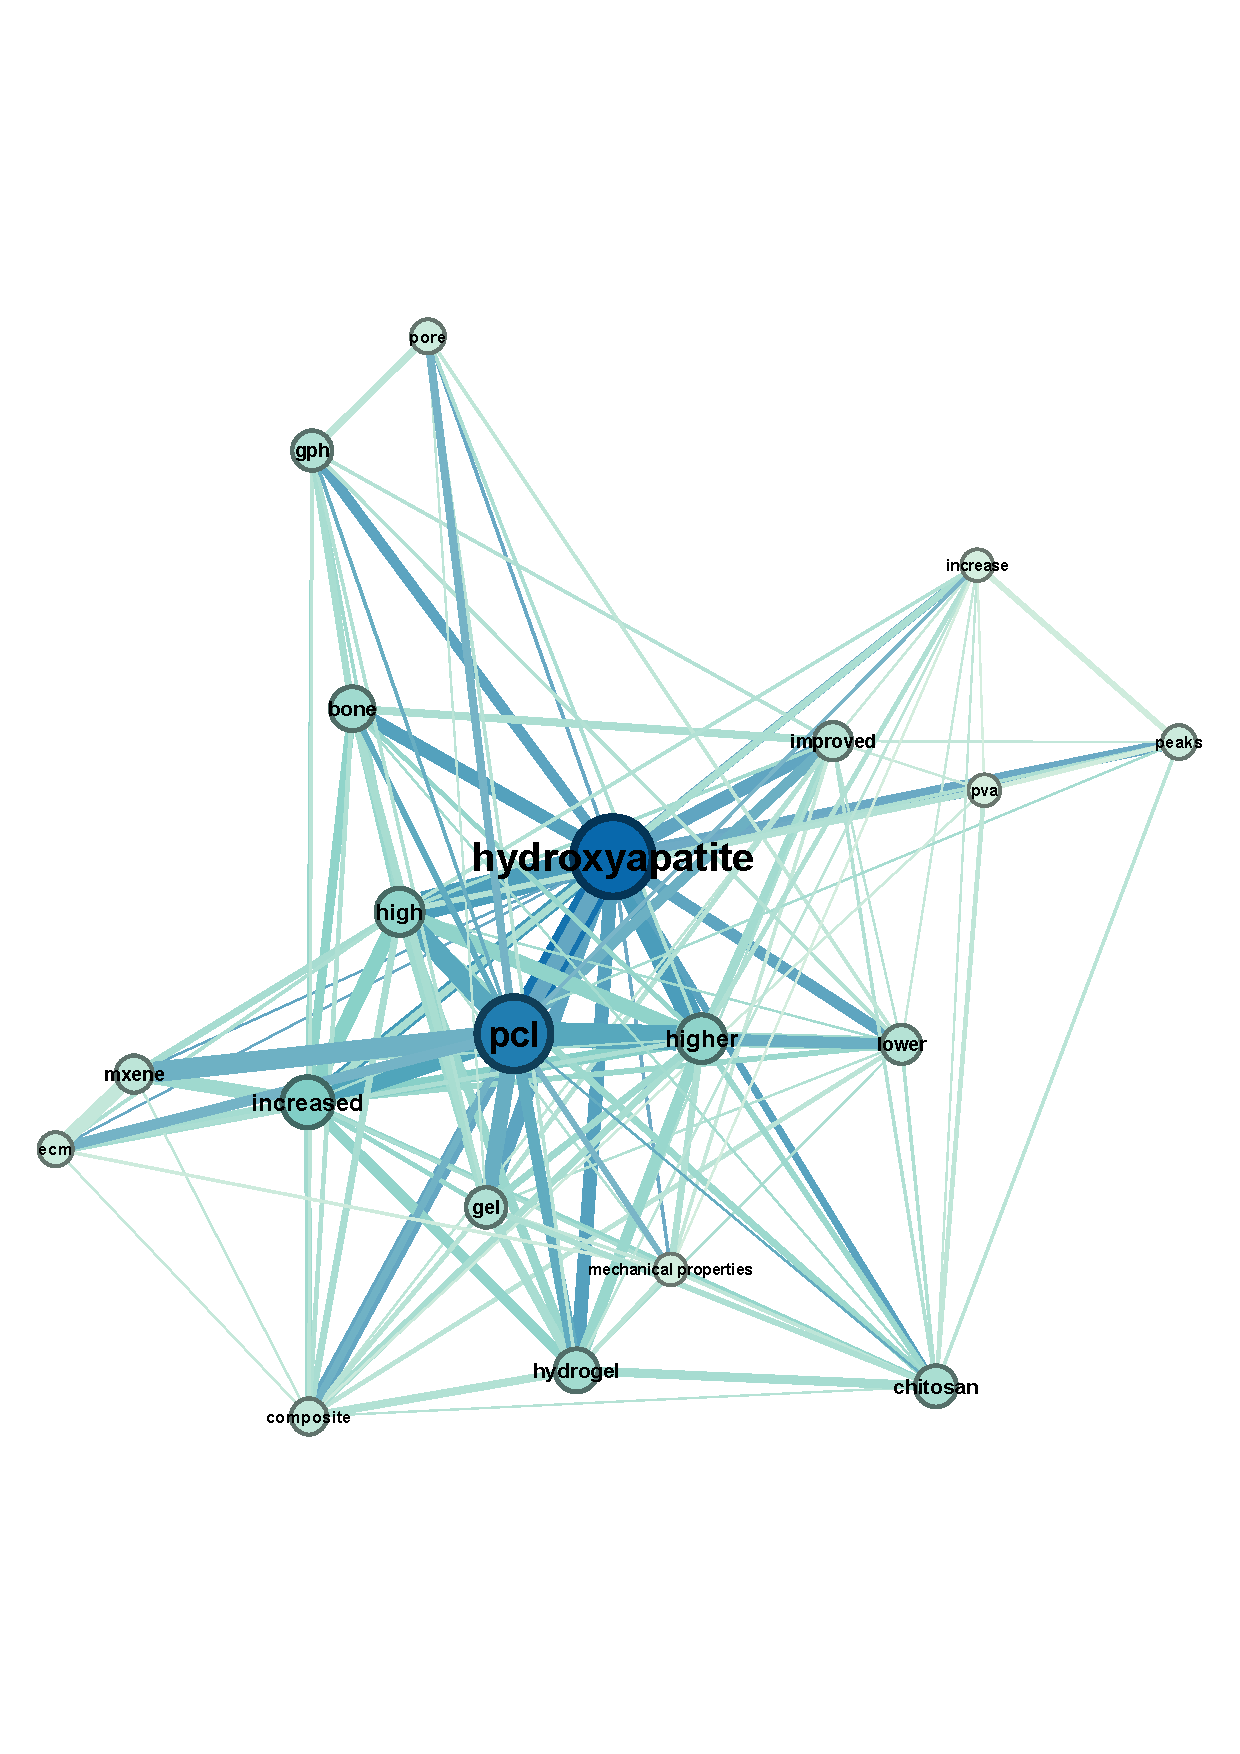
\includegraphics[width=0.85\linewidth,keepaspectratio]{figures/figura_red_material_composicion_gephi_crop.pdf}
\caption{Entity co-occurrence network for the Material/Composition content axis (1,035 nodes, 7,204 edges in the complete network), filtered to the most highly connected nodes for legibility; the complete network is provided as Supplementary Material (\texttt{.gexf}). Node size represents degree centrality; node color intensity represents betweenness centrality; edge thickness represents co-occurrence frequency.}
\label{fig:red_material}
\end{figure}

In the Fabrication Strategy network (590 nodes, 3,759 edges; Supplementary Material), PCL (degree 0.31; betweenness 0.32) bridges two distinct technological families: a polydopamine/nanoshell-mediated photothermal-modification cluster (PCL--polydopamine--gold nanoshells--near-infrared ablation) and a printing/bioink cluster (3D printing, biomaterial ink); hydroxyapatite (degree 0.31; betweenness 0.48), already under its normalized name, attains essentially the same degree as PCL while connecting substantially more efficiently to both clusters, especially the printing one, giving it a markedly higher betweenness than PCL despite the two now being nearly tied on degree --- consistent with hydroxyapatite acting as the more indispensable bridge between the two technological families even though PCL and hydroxyapatite now touch a comparable number of individual nodes overall. This quantitatively reinforces Section~\ref{sec:strategies}: modification-strategy combinations cluster into coherent technological families rather than occurring at random, with PCL and hydroxyapatite both versatile materials bridging these families.

In the Engineering Property network (378 nodes, 2,834 edges; Supplementary Material), PCL is the clearly dominant node on both measures (degree 0.43, betweenness 0.55), with hydroxyapatite a substantial but distinctly secondary hub (degree 0.34, betweenness 0.40); the two remain directly connected to each other. The presence of PVDF (a piezoelectric polymer) connected to this core, alongside calcium, suggests a subset of studies combining chemical bioactivity with electrical stimulation as a design strategy; two included studies independently support this pattern, combining PCL with piezoelectric PVDF or ceramic reinforcement under mechanical or electrical stimulation to enhance osteogenesis \cite{ref21,ref38} --- an angle only briefly developed in this review's narrative text and meriting further attention.

Figure~\ref{fig:red_funcion} shows the Biological Function network, the axis with the highest density of biological findings among the five. PCL is the dominant node by a wide margin (degree 0.41; betweenness 0.74, the single highest betweenness value observed across all five networks), with a strongly interconnected alkaline-phosphatase--calcium--bone cluster corresponding to standard osteogenic-differentiation markers. The presence of VEGF points to a vascularization sub-theme not currently developed in this review's narrative and represents a legitimate additional line of discussion, distinct from the bone-mineralization association already reported. Polydopamine (PDA) appears in this axis as well as in Fabrication Strategy; its co-occurrence with cell-adhesion and proliferation vocabulary is consistent with an active functional role rather than a purely passive structural one, though co-occurrence alone does not establish causation.

\begin{figure}[t]
\centering
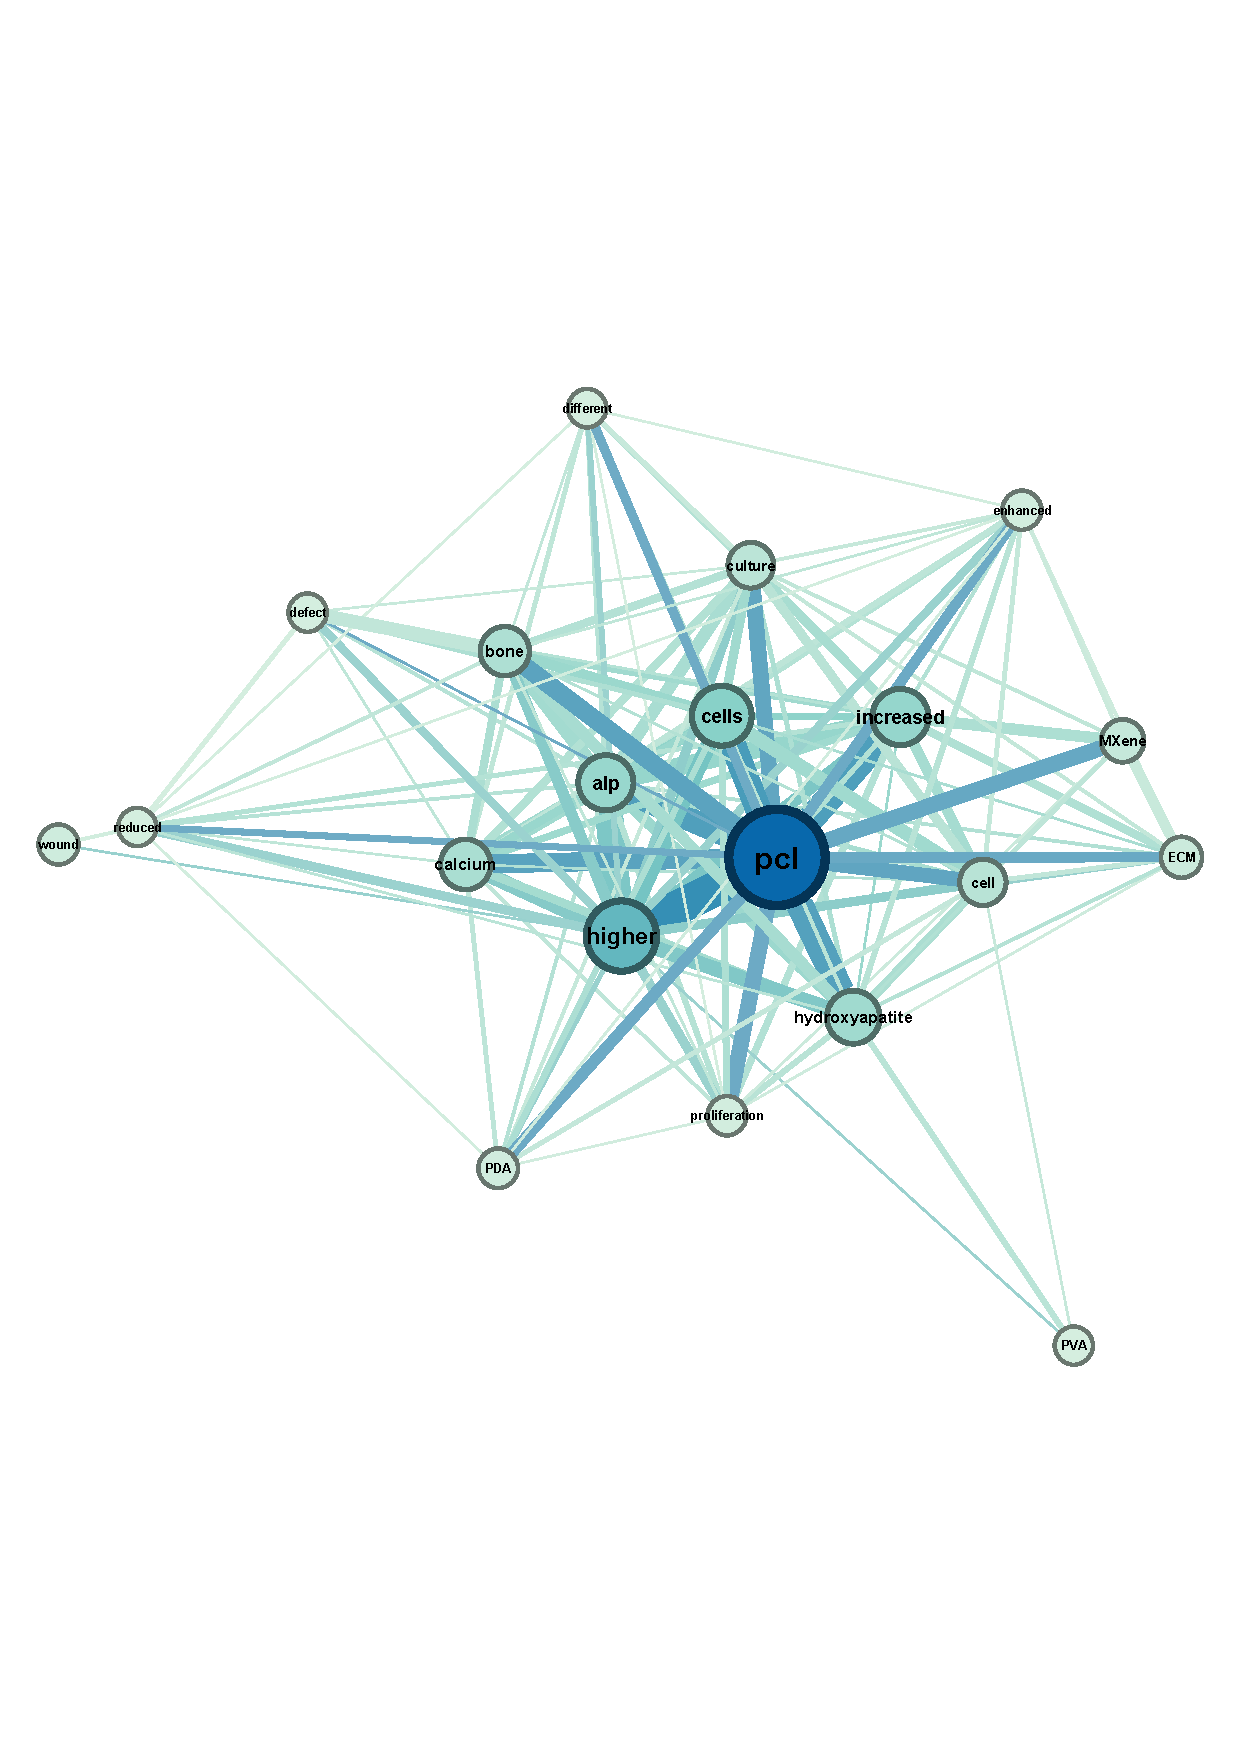
\includegraphics[width=0.85\linewidth,keepaspectratio]{figures/figura_red_funcion_biologica_gephi_crop.pdf}
\caption{Entity co-occurrence network for the Biological Function content axis (659 nodes, 3,324 edges in the complete network), filtered to the most highly connected nodes for legibility; the complete network is provided as Supplementary Material (\texttt{.gexf}). Node size represents degree centrality; node color intensity represents betweenness centrality; edge thickness represents co-occurrence frequency.}
\label{fig:red_funcion}
\end{figure}

Figure~\ref{fig:red_tissue} shows the Tissue Application network (483 nodes, 1,760 edges, the smallest and sparsest of the five; Supplementary Material). Bone dominates by both degree (0.30) and betweenness (0.56) by a clearly wider margin than in earlier reconstructions, and is directly connected to hydroxyapatite (degree 0.17; betweenness 0.25); its betweenness is still not the highest observed across the five networks (that distinction belongs to PCL in Biological Function, above). Hydroxyapatite and PCL (degree 0.17; betweenness 0.20) are now comparably central to each other in this axis, both clearly secondary to bone; tendon, which in an earlier reconstruction appeared as a close second to bone, is here a substantially smaller node (degree 0.12; betweenness 0.11) forming its own distinct, smaller cluster (collagen, bFGF, and related fibrous-tissue vocabulary) rather than visually rivaling the bone cluster in size. PCL retains its own soft-tissue cluster directly connected to meniscus, smooth muscle cells, elastin, and fiber-related nodes. Unlike in an earlier, uncorrected run of this analysis, the node ``wound'' is no longer isolated: it is now one of the axis's more connected nodes, with 59 edges (degree 0.12; betweenness 0.15), connecting sensibly to ``healing,'' ``wound healing,'' ``wound repair,'' and inflammation-related vocabulary --- confirming that its earlier apparent isolation was a pipeline artifact rather than a genuine feature of the data, and that this connectivity has strengthened further, not merely persisted, under the corrected pipeline.

\begin{figure}[t]
\centering
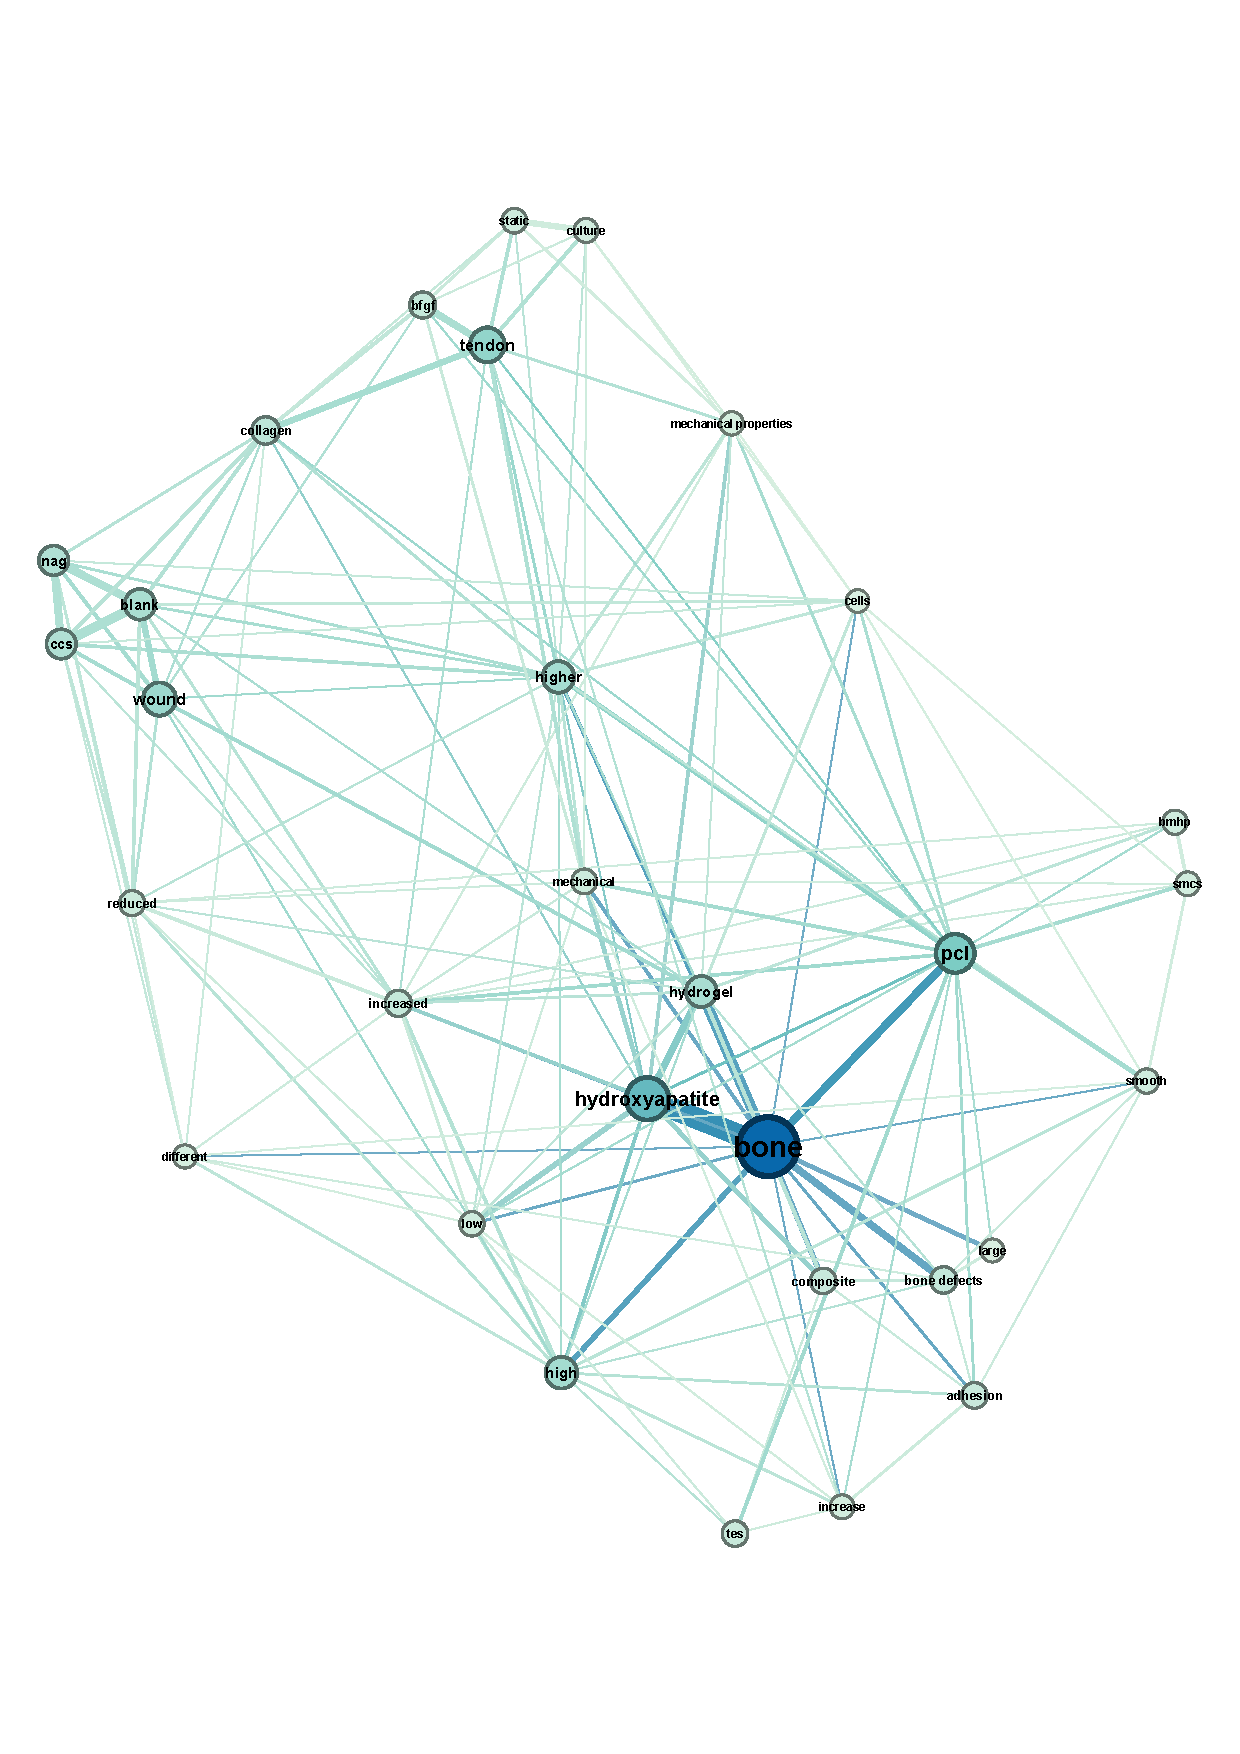
\includegraphics[width=0.85\linewidth,keepaspectratio]{figures/figura_red_aplicacion_tisular_gephi_crop.pdf}
\caption{Entity co-occurrence network for the Tissue Application content axis (483 nodes, 1,760 edges in the complete network), filtered to the most highly connected nodes for legibility; the complete network is provided as Supplementary Material (\texttt{.gexf}). Node size represents degree centrality; node color intensity represents betweenness centrality; edge thickness represents co-occurrence frequency.}
\label{fig:red_tissue}
\end{figure}

The five networks were built from a shared, non-exclusive axis assignment --- a single fragment can satisfy more than one axis condition and so can contribute to more than one network --- so they are not independent replications on disjoint data, and their agreement should not be read as independent statistical confirmation. With that caveat, the pattern across axes is more mixed than a clean bioactivity-versus-mechanical-support division would predict. Hydroxyapatite is the most central node in Material/Composition and connects directly to bone in Tissue Application, consistent with a compositional and osteoconductive role. PCL, however, is the most central node in Fabrication Strategy and, counterintuitively, is also the dominant node in Biological Function, where it is more strongly connected than hydroxyapatite to each member of the alkaline-phosphatase--calcium--bone cluster of osteogenic-differentiation markers (co-occurrence edge weights of 21, 17, and 16 for PCL versus 10, 7, and 10 for hydroxyapatite, respectively); the VEGF-associated vascularization vocabulary in this same axis is likewise connected only to PCL between the two (edge weight 16), not to hydroxyapatite at all. In Engineering Property, the axis most directly tied to mechanical/structural characterization, PCL is in fact clearly ahead of hydroxyapatite rather than co-equal with it (degree 0.43 for PCL versus 0.34 for hydroxyapatite; betweenness 0.55 versus 0.40), so PCL is now the more central node in three of the five axes (Fabrication Strategy, Engineering Property, and Biological Function), with hydroxyapatite leading only Material/Composition and the two materials comparably secondary to bone in Tissue Application. This pattern most plausibly reflects that PCL is both the most frequent principal material in this corpus (30/78 studies) and the material most often combined with a bioactive or osteogenic-signaling additive as a modification strategy (Section~\ref{sec:strategies}), so PCL's co-occurrence footprint captures a large share of this corpus's biological-function vocabulary through those additives rather than reflecting an intrinsic bioactivity of PCL itself; because this network analysis reflects textual co-occurrence rather than a demonstrated biological mechanism, it cannot by itself distinguish these two explanations. Rather than confirming a clean, materially intrinsic bioactivity/mechanical-support split, this network evidence is disclosed here as a genuine divergence from that simpler framing --- and from the distinct, quantitatively grounded material--outcome associations reported in Sections~\ref{sec:strategies}--\ref{sec:biocompat} (hydroxyapatite: osteogenic outcomes; PCL: mechanical stability), which are derived from studies' directly reported results rather than from text co-occurrence --- and is reported as such rather than reconciled with it after the fact. The reconstructed five-axis scheme also constitutes a methodologically more defensible alternative to the original $k$-means macro-grouping, since it avoids forcing an exclusive partition onto data with weak natural separation under that scheme (macro-group silhouette consistently $\approx$0.09 --- 0.092 for the original topics, 0.090 for the reconstructed topics --- regardless of how well-separated the underlying topic embeddings themselves are) without discarding the better-separated topic-level structure obtained with a fixed seed (silhouette $=0.52$ at the BERTopic stage).

\section{Discussion}
\label{sec:discussion}

This review synthesized evidence from 78 studies published since 2023 on hydroxyapatite-, chitosan-, and PCL-based tissue engineering scaffolds. The results suggest that no single material is categorically ``more biocompatible'' in an absolute sense; rather, each material's characteristic strength (osteoconductivity for hydroxyapatite, cell adhesion/antibacterial activity for chitosan, mechanical stability for PCL) aligns with a different aspect of scaffold performance, and the choice of material is better framed as a trade-off matched to the intended tissue application than as a single ranked hierarchy, consistent with prior reviews directly comparing these same three materials \cite{ref83}.

Interpreting the Material $\times$ Strategy $\times$ Tissue $\times$ Outcome $\times$ Evidence-Type matrix (Supplementary Table~S3) clarifies where this evidence base is strongest. At the \emph{material} level, PCL, chitosan, and hydroxyapatite recur with the functional associations described above; at the \emph{modification-strategy} level, nanoparticle incorporation, crosslinking, surface functionalization, and growth factor loading are the most frequently represented approaches (Section~\ref{sec:strategies}), often combined with \emph{architectural} choices such as pore size, fiber alignment, or printing pattern. As reported in Section~\ref{sec:biocompat}, the evidence base is substantially weighted toward bone-related applications and toward in-vitro-only evidence (51 of 78 studies); the observed material--strategy relationships should therefore not be assumed to generalize across tissue types or to in-vivo performance, particularly where evidence remains sparse.

\textbf{Novelty.} This review's contribution is not the individual coverage of hydroxyapatite, chitosan, or PCL scaffolds, each already reviewed separately in the recent literature \cite{ref80,ref81,ref82}, but the combination of: (i) a recent, cross-material synthesis spanning all three focus materials within a single evidence base; (ii) systematic mapping of modification strategies across materials rather than within a single-material review; (iii) a systematically re-examined and per-study-categorized concentration--response pattern across 19 candidate studies, distinguishing genuine non-monotonic responses from boundary effects, composition/formulation comparisons, and cross-outcome trade-offs (Section~\ref{sec:pattern}); (iv) the structured Material $\times$ Strategy $\times$ Tissue $\times$ Outcome $\times$ Evidence-Type synthesis (Supplementary Table~S3) enabling this cross-cutting interpretation; and (v) a complementary computational text-mining perspective on the same corpus (Section~4). Reference~\cite{ref83} is the closest recent overlap, as it also addresses PCL, chitosan, and hydroxyapatite in combination; however, it is a narrative review focused specifically on ternary PCL-chitosan-hydroxyapatite composite systems, without a systematic search protocol, PRISMA-guided study selection, or a structured cross-study extraction matrix. By contrast, the present review applies a PRISMA 2020 protocol, considers the three materials both individually and in combination, and reports a structured, auditable Material $\times$ Strategy $\times$ Tissue $\times$ Outcome $\times$ Evidence-Type extraction (Supplementary Table~S3) rather than a narrative synthesis.

Two sub-themes surfaced by the data-driven analysis (Section~\ref{sec:q3}) but not fully developed above merit brief mention. First, PCL combined with piezoelectric PVDF or ceramic reinforcement under mechanical/electrical stimulation recurred as a bioelectric strategy for enhancing osteogenesis in at least two studies \cite{ref21,ref38}, an underexplored complement to Section~\ref{sec:strategies}'s chemical and structural strategies. Second, a VEGF-associated vascularization sub-theme in the Biological Function network is distinct from the bone-mineralization associations dominating this evidence base; a VEGF-mimetic peptide was among the growth factors loaded in Section~\ref{sec:strategies} \cite{ref77}, indicating vascularization strategies remain comparatively underrepresented relative to osteogenic outcomes.

\textbf{Limitations.} This review has several limitations. It was not prospectively registered (e.g., PROSPERO) and no protocol was published in advance of the search (Section~2.1); although eligibility criteria and search strategy were fixed before full-text screening began, this cannot be independently verified without a public, time-stamped protocol. The search was restricted to two databases (Scopus and Web of Science); PubMed/MEDLINE and Embase index somewhat different subsets of the biomedical literature, so a third database could improve recall in future work (Section~2.7). Full-text accessibility was a predefined Stage 2 eligibility criterion (Section~2.4): 37 of the 124 records sought could not be retrieved and were excluded without content-based assessment, which may have introduced availability-related selection bias favoring journals or institutions with broader open-access coverage; the remaining 87 records were assessed, of which 9 were excluded for the content-based reasons in Table~\ref{tab:excl}. Full-text screening was performed by a single reviewer rather than independently by two, which may increase the risk of selection and extraction errors relative to dual independent screening.

A formal risk-of-bias assessment was applied to all 78 included studies against the full text of each article: the QUIN tool (12 items, originally developed and validated for in vitro dental-material studies) for the in vitro component of every study --- chosen in the absence of a validated risk-of-bias tool specific to in vitro biomaterials or tissue-engineering research, and applied here without modification to its items, since its 12 criteria (sample-size justification, randomization, blinding, comparison-group definition, outcome standardization, statistical reporting) are methodologically generic rather than anatomically dental-specific, with generic wording (e.g., ``sampling technique and eligibility described'') interpreted at the level of the cell/scaffold groups described in each study rather than dental specimens specifically --- and the SYRCLE tool (10 domains) for the 27 studies with an in vivo or chorioallantoic-membrane (CAM) component, with each item/domain judged Yes/No/Unclear and an overall Low risk/Some concerns/High risk rating assigned per study and per tool (Supplementary Table~S5), as neither tool prescribes a fixed algorithm for this step (Hooijmans et al., 2014). An internal consistency audit of the initial, qualitative overall judgements found that a substantial number of studies sharing an identical or near-identical item-level profile had nonetheless received different overall ratings; an explicit, uniform threshold was therefore adopted to resolve this regardless of which rating a given study had initially received: a study was rated Some concerns only when at least 8 of the 12 QUIN items, or 4 of the 10 SYRCLE domains, were rated Yes, and High risk otherwise. One SYRCLE domain (D4, random housing, which presumes a live-animal housing environment) was judged not applicable to the 2 CAM (chorioallantoic-membrane) studies and excluded from those two studies' Yes-count and overall judgement rather than forced to Yes, No, or Unclear. Across the 78 studies scored with QUIN, 7 were rated Some concerns and 71 High risk, with no study rated Low risk, driven mainly by the near-universal absence of sample-size justification, operator/assessor detail, randomization, and blinding despite otherwise clear aims, controls, methodology, and statistics. Among the 27 studies with an in vivo or CAM component, SYRCLE ratings were similarly skewed toward High risk (25 of 27) and Some concerns (2 of 27), driven by unreported allocation concealment, random housing, and blinding even where randomization to groups was stated. To check inter-rater reliability, this assessment was independently repeated in full by a second, blinded assessor across all 78 studies prior to the consistency audit described above; the second assessor reached the same overall judgement as the first for every study under both tools, substantially mitigating the single-reviewer screening limitation above, though item-level concordance was not additionally quantified with a formal statistic such as Cohen's kappa, so this is reported as a qualitative dual-assessment check that predates, and was not re-verified against, the threshold-based correction above. A simplified, non-validated reporting-quality indicator computed independently from the extraction summary (0--4; Supplementary Table~S2, scoring whether variability, a comparison group, statistical significance, and a quantitative value with units were reported) shows a consistent pattern (1 of 78 studies reported all four elements, 36 reported two or three, 41 reported zero or one), converging with the formal QUIN/SYRCLE assessment on the same overall picture: incomplete methodological reporting is widespread across this primary literature, not only a limitation of the present analysis. Future primary studies in this field would benefit from standardized reporting of sample size, randomization, blinding, operator/assessor detail, variability, controls, statistical methods, and quantitative values with units. The full extraction matrix, indicator scores, and risk-of-bias ratings are provided as Supplementary Tables~S1, S2, and S5 to support auditability of the synthesis.

\section{Conclusion}

This systematic review synthesized evidence from 78 studies on hydroxyapatite-, chitosan-, and PCL-based tissue engineering scaffolds. No single material was categorically superior in an absolute sense; rather, each exhibited a distinct performance strength --- osteoconductivity for hydroxyapatite, cell adhesion and antibacterial activity for chitosan, and mechanical stability for PCL --- indicating that material selection should be guided by the intended tissue application rather than a universal hierarchy. These performance strengths reflect predominantly in vitro, formulation- and modification-specific evidence (51 of the 78 included studies were in vitro only); because all 30 PCL studies included at least one modification strategy, these conclusions do not extend to unmodified PCL, and should be read as conditional on tissue type, experimental model, and the reporting quality of the underlying studies rather than as general design rules. Among modification strategies, nanoparticle incorporation, surface functionalization, crosslinking, structural design, growth factor loading, and drug loading all demonstrated quantifiable effects, with a concentration-dependent response pattern observed across a subset of studies, though on systematic re-examination only part of this subset (7 of 14 studies with a genuine dose series) reflects a true non-monotonic, interior-optimum response, while the remainder reflects a boundary effect, a composition/formulation comparison, or a cross-outcome trade-off (Section~\ref{sec:pattern}). A complementary data-driven network analysis, applying a methodologically distinct approach to the same corpus, did not find a clean bioactivity-versus-mechanical-support division between these two materials: hydroxyapatite was the most conceptually central material overall and the one most directly linked to bone, whereas PCL was unexpectedly the most central node in the fabrication-strategy, engineering-property, and biological-function axes alike, plausibly reflecting its frequency in this corpus and its common combination with bioactive additives rather than an intrinsic mechanical-only role, with the two materials comparably central to each other only in the tissue-application axis, where bone was the dominant node overall; this network analysis also identified structurally significant bridge concepts warranting further investigation. Future reviews could extend the search to a third bibliographic database and further explore the underexplored cross-cutting concepts identified here.

\section*{Declarations}

\subsection*{CRediT Authorship Contribution Statement}

\textbf{Ethan Nicolás García San Andrés:} Conceptualization, Methodology, Software, Formal analysis, Investigation, Data curation, Writing -- original draft, Visualization. \textbf{Juan Carlos García Plúa:} Conceptualization, Supervision, Writing -- review \& editing.

\subsection*{Funding}

This research received no external funding.

\subsection*{Declaration of Competing Interest}

The authors declare no conflict of interest.

\subsection*{Data Availability}

The data extraction dataset supporting the findings of this review (search exports, deduplication logs, and the standardized extraction table for the 78 included studies) is available as supplementary material and at the corresponding author's GitHub repository (\seqsplit{https://github.com/Ethnign/Biomaterial-Scaffold-Design-for-Tissue-Engineering-A-Data-Driven-Systematic-Review-Repository}), version \texttt{v1.0.0}, the citable snapshot corresponding to this manuscript. The full per-study extraction matrix (Supplementary Table~S1), reporting-quality indicator scores (Supplementary Table~S2), and the Material $\times$ Strategy $\times$ Tissue $\times$ Outcome $\times$ Evidence-Type matrix (Supplementary Table~S3) for all 78 included studies, together with the concentration-level detail and per-study response categorization for the 19 studies examined for the concentration--response pattern (Supplementary Table~S4, Section~\ref{sec:pattern}) and the QUIN/SYRCLE risk-of-bias assessment for all 78 included studies (Supplementary Table~S5, Section~\ref{sec:discussion}), are provided in the same repository.

\subsection*{Acknowledgements}

Not applicable.

\subsection*{Declaration of Generative AI and AI-Assisted Technologies in the Manuscript Preparation Process}

During the preparation of this work, the authors used Claude (Anthropic) as a complementary assistive tool for literature search support, data extraction and formatting, development of statistical and natural language processing code, and generation of the graphical abstract illustration. Every AI-assisted literature search result, extracted data point, code output, reference, and image was independently verified by the authors against the primary source before inclusion; discrepancies identified during verification were corrected by the authors. AI was not used for scientific interpretation, conclusions, or decision-making, and is not listed as an author. After using this tool, the authors reviewed and edited the content as needed and take full responsibility for the content of the published work.



\begin{thebibliography}{78}
\fontsize{5.5}{6.0}\selectfont
\setlength{\itemsep}{0pt}
\setlength{\parsep}{0pt}
\setlength{\parskip}{0pt}
\bibitem{ref1} Li Y.; Li H.; Bian P.-Y., et al. Research on the performance of HAP/ALG composite bone scaffolds with bone unit structure. International Journal of Biological Macromolecules. 2026. doi:10.1016/j.ijbiomac.2026.150751
\bibitem{ref2} Naolou T.; Schadzek N.; Hornbostel J.M., et al. Enhanced gelatin methacryloyl nanohydroxyapatite hydrogel for high-fidelity 3D printing of bone tissue engineering scaffolds. Biofabrication. 2025. doi:10.1088/1758-5090/adbb90
\bibitem{ref3} Mitropoulou A.; Markatos D.N.; Dimopoulos A., et al. Development and Evaluation of Biodegradable Core-Shell Microfibrous and Nanofibrous Scaffolds for Tissue Engineering Applications. Journal of Materials Science: Materials in Medicine. 2024. doi:10.1007/s10856-024-06777-z
\bibitem{ref4} Hosseini M.; Najmoddin N.; Zamanlouie S. 3D printed biomimetic nanocomposite scaffold with potential osteo-neurogenic differentiation of mesenchymal stem cells for bone repair. Chemical Engineering Journal Advances. 2026. doi:10.1016/j.ceja.2026.101100
\bibitem{ref5} Zhou K.; Azaman F.A.; Cao Z., et al. Bone Tissue Engineering Scaffold Optimisation through Modification of Chitosan/Ceramic Composition. Macromol. 2023. doi:10.3390/macromol3020021
\bibitem{ref6} Cui Y.; Xu J.; Gu X., et al. Development of magnetic field induced ordered magnetoelectric bifunctional bone tissue engineering scaffold. Materials Letters. 2026. doi:10.1016/j.matlet.2025.139689
\bibitem{ref7} Song S.; Guo J.; Kong B., et al. Black phosphorus-loaded anisotropic nanofiber sponges for random skin flaps regeneration. Chemical Engineering Journal. 2024. doi:10.1016/j.cej.2024.158133
\bibitem{ref8} Shen W.; Mao Y.; Ge X., et al. PLA tissue-engineered scaffolds loaded with sustained-release active substance chitosan nanoparticles: Modeling BSA-bFGF as the active substance. International Journal of Biological Macromolecules. 2024. doi:10.1016/j.ijbiomac.2024.133120
\bibitem{ref9} Wang J.; Huang G.; Qin Q., et al. Performance study of ZnO-TPU/CS bilayer composite electrospinning scaffold in skin wound healing. Frontiers in Bioengineering and Biotechnology. 2025. doi:10.3389/fbioe.2025.1636932
\bibitem{ref10} Zhao W.; Yang Y.; Liu Y., et al. Biomimetic multilayer scaffolds with prolonged retention of stem cells-recruiting and angiogenic peptides for promoting bladder regeneration. Composites Part B: Engineering. 2024. doi:10.1016/j.compositesb.2024.111409
\bibitem{ref11} Wu H.; Zhong X.; Leng P., et al. 3D-printed oxygen-releasing scaffolds promote bone repair via angiogenesis and osteogenesis. APL Materials. 2025. doi:10.1063/5.0305073
\bibitem{ref12} Nabizadeh Z.; Nasrollahzadeh M.; Heidari F., et al. A drug-loaded nano chitosan/hyaluronic acid hydrogel system as a cartilage tissue engineering scaffold for drug delivery. International Journal of Biological Macromolecules. 2024. doi:10.1016/j.ijbiomac.2024.137314
\bibitem{ref13} You C.; Zhu Z.; Wang S., et al. Nanosilver alleviates foreign body reaction and facilitates wound repair by regulating macrophage polarization. Journal of Zhejiang University: Science B. 2023. doi:10.1631/jzus.B2200447
\bibitem{ref14} Wang Y.; Zhou X.; Jiang J., et al. Carboxymethyl chitosan-enhanced multi-level microstructured composite hydrogel scaffolds for bone defect repair. Carbohydrate Polymers. 2025. doi:10.1016/j.carbpol.2024.122847
\bibitem{ref15} Zeng J.; Li W.; Li Y., et al. A chitosan-based composite scaffold as a bioactive strontium-delivery system mediating accelerated bone regeneration. Carbohydrate Polymers. 2026. doi:10.1016/j.carbpol.2026.125082
\bibitem{ref16} Sheng N.; Lin W.; Lin J., et al. Cross-linking manipulation of waterborne biodegradable polyurethane for constructing mechanically adaptable tissue engineering scaffolds. Regenerative Biomaterials. 2024. doi:10.1093/rb/rbae111
\bibitem{ref17} Shlomo-Avitan B.; Machour M.; Ahmad S.S., et al. Emulsion-templated macroporous polycaprolactone: Synthesis, degradation, additive manufacturing, and cell-growth. Polymer. 2025. doi:10.1016/j.polymer.2024.127971
\bibitem{ref18} Farnaghi M.; Poursamar S.A.; Farzan M., et al. Enhancing the biological characteristics of aminolysis surface-modified 3D printed nanocomposite polycaprolactone/nanohydroxyapatite scaffold via gelatin biomacromolecule immobilization: An in vitro and in vivo study. Colloids and Surfaces B: Biointerfaces. 2025. doi:10.1016/j.colsurfb.2025.114505
\bibitem{ref19} Tang W.; Pan P.; Chen T., et al. 3D chitosan scaffolds loaded with ZnO nanoparticles for bone tissue engineering. Colloids and Surfaces B: Biointerfaces. 2025. doi:10.1016/j.colsurfb.2024.114199
\bibitem{ref20} Moreno M.; Devi A.; Zanders D., et al. Ti-metalation of chitosan films by VPM, MPI and PEALD processes: An avenue to antiseptic scaffolds and functional biopolymers. Applied Surface Science Advances. 2026. doi:10.1016/j.apsadv.2026.100963
\bibitem{ref21} Asadi G.; Katbab A.A.; Bagheri-khoulenjani S., et al. Piezoelectric PCL/PVDF core-shell nanofibrous scaffolds for enhanced osteogenesis under dynamic loading. Biomaterials Advances. 2026. doi:10.1016/j.bioadv.2026.214888
\bibitem{ref22} Biju R.F.; Samy S.A.D.; G J., et al. Physicochemical, mechanical, antibacterial and cytotoxicity evaluation of hydroxyapatite anchored ZnO and CuO as potential composite biomaterials. Ceramics International. 2026. doi:10.1016/j.ceramint.2026.05.176
\bibitem{ref23} Ma S.; Zhang L.; Wu Y., et al. Glucosamine sulfate-loaded nanofiber reinforced carboxymethyl chitosan sponge for articular cartilage restoration. Journal of Colloid and Interface Science. 2025. doi:10.1016/j.jcis.2024.07.207
\bibitem{ref24} Delemeester M.; Pawelec K.M.; Hix J.M.L., et al. Device Design and Advanced Computed Tomography of 3D Printed Radiopaque Composite Scaffolds and Meniscus. Advanced Functional Materials. 2024. doi:10.1002/adfm.202404860
\bibitem{ref25} Salehi S.; Ghomi H.; Hassanzadeh-Tabrizi S.A., et al. Antibacterial and osteogenic properties of chitosan-polyethylene glycol nanofibre-coated 3D printed scaffold with vancomycin and insulin-like growth factor-1 release for bone repair. International Journal of Biological Macromolecules. 2025. doi:10.1016/j.ijbiomac.2025.139883
\bibitem{ref26} Mitra I.; Potes M.A.; Shafi M., et al. Enzyme-delivery Metal-organic Framework Composite Coatings for Restoration of Hyperglycemia-damaged Osteoblast Differentiation. Biomaterials Advances. 2025. doi:10.1016/j.bioadv.2024.214055
\bibitem{ref27} Madaninasab P.; Ebrahimian-Hosseinabadi M.; Zargar Kharazi A. Polycaprolactone/retinoic acid/nano-hydroxyapatite composites for neural tissue engineering. Materials Chemistry and Physics. 2026. doi:10.1016/j.matchemphys.2026.132269
\bibitem{ref28} Ucan M.T.; Meng D.; Aslan E., et al. Design, Fabrication, and Evaluation of Hybrid Polycaprolactone/Graphene Scaffold Based on Additive Manufacturing and Electrospinning. Macromolecular Materials and Engineering. 2025. doi:10.1002/mame.202500236
\bibitem{ref29} Shen G.; Gao B.; Guo J., et al. Dynamic culturing of large cell-loaded PCL/gelatin methacryloyl scaffolds for bone critical size defect repair. International Journal of Biological Macromolecules. 2025. doi:10.1016/j.ijbiomac.2025.139906
\bibitem{ref30} Mirzavandi Z.; Poursamar S.A.; Amiri F., et al. 3D printed polycaprolactone/gelatin/ordered mesoporous calcium magnesium silicate nanocomposite scaffold for bone tissue regeneration. Journal of Materials Science: Materials in Medicine. 2024. doi:10.1007/s10856-024-06828-5
\bibitem{ref31} Ali S.M.; Gomaa E.H.; Badr E.E., et al. Nanobioactive glass/chitosan/collagen composite loaded with methylene blue for tissue regeneration and bacterial infection treatment by photodynamic therapy. Journal of Photochemistry and Photobiology B: Biology. 2025. doi:10.1016/j.jphotobiol.2025.113179
\bibitem{ref32} Liu H.; Wang C.; Zheng L., et al. 3D-Architected Natural Tooth-Derived Scaffolds Reinforced by Graphene and Gradient Gyroid. Small Structures. 2025. doi:10.1002/sstr.202500498
\bibitem{ref33} Li Z.; Chen R.; Hao Z., et al. Hydrogel inspired by "adobe" with antibacterial and antioxidant properties for diabetic wound healing. Materials Today Bio. 2025. doi:10.1016/j.mtbio.2025.101477
\bibitem{ref34} Jones A.J.; Carothers L.A.; Paez F., et al. 3D-Printed Biocompatible Frames for Electrospun Nanofiber Membranes: An Enabling Biofabrication Technology for Three-Dimensional Tissue Models and Engineered Cell Culture Platforms. Micromachines. 2025. doi:10.3390/mi16080887
\bibitem{ref35} Wang M.; Liu H.; Zhao W., et al. Design and Characterization of Curcumin-Modified Polyurethane Material with Good Mechanical, Shape-Memory, pH-Responsive, and Biocompatible Properties. Biomolecules. 2025. doi:10.3390/biom15081070
\bibitem{ref36} Cinici B.; Gozonunde S.; Kurt M., et al. Development of Polylactic Acid/Hydroxyapatite Composite Filaments for 3D Printing of Bone Tissue Engineering Scaffolds. Progress in Biomaterials. 2025. doi:10.57647/pibm.2025.17542
\bibitem{ref37} Salehi R.; Ebrahimian-Hosseinabadi M.; Rafienia M. Fabrication and characterization of polycaprolactone/chitosan/graphene quantum dots nanocomposite scaffolds with potential application in neural tissue engineering. Carbon Trends. 2025. doi:10.1016/j.cartre.2025.100595
\bibitem{ref38} Meng D.; Hou Y.; Zubairi H., et al. Ceramic-based piezoelectric material reinforced 3D printed polycaprolactone bone tissue engineering scaffolds. Materials and Design. 2025. doi:10.1016/j.matdes.2025.114542
\bibitem{ref39} Kang J.; Shirzad M.; Ranganathan P., et al. Suspended 3D printing of polycaprolactone/ hydroxyapatite composites for the fabrication of complex bone scaffolds. International Journal of Bioprinting. 2025. doi:10.36922/IJB025320319
\bibitem{ref40} Krishani M.; Chong J.N.; Lim W.R., et al. Synthesis and Characterization of Keratin-Based Scaffold for Potential Tissue Engineering Applications. Fibers. 2025. doi:10.3390/fib13070097
\bibitem{ref41} Gepek E.; Fayyazbakhsh F.; Suliandziga L., et al. PLA-based bone tissue engineering scaffolds incorporating hydroxyapatite and bioactive glass using digital light processing. International Journal of Bioprinting. 2025. doi:10.36922/IJB025040029
\bibitem{ref42} Huang S.; Wang Z.; Sun X., et al. Bone Morphogenetic Protein 7-Loaded Gelatin Methacrylate/Oxidized Sodium Alginate/ Nano-Hydroxyapatite Composite Hydrogel for Bone Tissue Engineering. International Journal of Nanomedicine. 2024. doi:10.2147/IJN.S461996
\bibitem{ref43} Zhu S.S.; Sun H.N.; Mu T.H., et al. Cellulose nano-dispersions enhanced by ultrasound assisted chemical modification drive osteoblast proliferation and differentiation in PVA/HA bone tissue engineering scaffolds. International Journal of Biological Macromolecules. 2024. doi:10.1016/j.ijbiomac.2024.135571
\bibitem{ref44} Howard C.J.; Paul A.; Duruanyanwu J., et al. The Manufacturing Conditions for the Direct and Reproducible Formation of Electrospun PCL/Gelatine 3D Structures for Tissue Regeneration. Nanomaterials. 2023. doi:10.3390/nano13243107
\bibitem{ref45} Peng H.R.; Zhao Q.; Xiao T., et al. Preparation and properties of magnesium/strontium modified hydroxyapatite whisker bone tissue engineering scaffold. Materials Letters. 2024. doi:10.1016/j.matlet.2024.135922
\bibitem{ref46} Najar S.M.; Seyedjafari E.; Nemati F., et al. Osteogenic differentiation of human adipose-derived stem cells on polycaprolactone 3D-printed scaffolds containing bioactive bioceramic. Materialia. 2024. doi:10.1016/j.mtla.2024.102051
\bibitem{ref47} Ge J.H.; Drees R.; Wang A.R., et al. Micron-Sized Fe3O4/PCL Biocomposite Scaffolds to Attract Magnetic Nanoparticles for Targeted Drug Delivery. Bioengineering (Basel). 2025. doi:10.3390/bioengineering12040371
\bibitem{ref48} Qing J.; Tan J.W.; Xiao T., et al. Directional extrusion preparation and properties of ordered porous gelatin/nano-hydroxyapatite bone tissue engineering scaffolds. Materials Letters. 2025. doi:10.1016/j.matlet.2025.138351
\bibitem{ref49} Wang X.F.; Zou Z.F.; Li K.C., et al. Design and fabrication of dual-layer PCL nanofibrous scaffolds with inductive influence on vascular cell responses. Colloids and Surfaces B: Biointerfaces. 2024. doi:10.1016/j.colsurfb.2024.113988
\bibitem{ref50} Ghadirian S.; Shariati L.; Karbasi S. Evaluation of the effects of cartilage decellularized ECM in optimizing PHB-chitosan-HNT/chitosan-ECM core-shell electrospun scaffold: Physicochemical and biological properties. Biomaterials Advances. 2025. doi:10.1016/j.bioadv.2025.214249
\bibitem{ref51} Pan P.; Wang J.; Wang X., et al. Physically cross-linked chitosan gel with tunable mechanics and biodegradability for tissue engineering scaffold. International Journal of Biological Macromolecules. 2024. doi:10.1016/j.ijbiomac.2023.128682
\bibitem{ref52} Jia Z.L.; Ma H.L.; Liu J.Q., et al. Preparation and Characterization of Polylactic Acid/Nano Hydroxyapatite/Human Acellular Amniotic Membrane (PLA/nHAp/HAAM) Hybrid Scaffold for Bone Tissue Defect Repair. Materials. 2023. doi:10.3390/ma16051937
\bibitem{ref53} Su Y.C.; Zhang Y.G.; Chen Y., et al. Surface recrystallization on melt electrowritten scaffolds for acceleration of osteogenic differentiation. Materials Today Physics. 2024. doi:10.1016/j.mtphys.2024.101344
\bibitem{ref54} Jamali S.A.; Mohammadi M.; Saeed M., et al. Biomimetic fiber/hydrogel composite scaffolds based on chitosan hydrogel and surface modified PCL chopped-microfibers. International Journal of Biological Macromolecules. 2024. doi:10.1016/j.ijbiomac.2024.134936
\bibitem{ref55} Woods I.; Spurling D.; Sunil S., et al. 3D-Printing of Electroconductive MXene-Based Micro-Meshes in a Biomimetic Hyaluronic Acid-Based Scaffold Directs and Enhances Electrical Stimulation for Neural Repair Applications. Advanced Science. 2025. doi:10.1002/advs.202503454
\bibitem{ref56} Bhattacharyya A.; Ham H.W.; Sonh J., et al. 3D bioprinting of complex tissue scaffolds with in situ homogeneously mixed alginate-chitosan-kaolin bioink using advanced portable biopen. Carbohydrate Polymers. 2023. doi:10.1016/j.carbpol.2023.121046
\bibitem{ref57} Jagitay M.B.; Ustundag G.; Celik Z.D., et al. 3D printing of olive pit powder-reinforced PVA/HAp scaffolds: a sustainable strategy for bone tissue engineering. Polymer Bulletin. 2026. doi:10.1007/s00289-026-06303-x
\bibitem{ref58} Zhang X.X.; Ouyang J.F.; Li B.Q., et al. Novel fabrication of self-healing chitosan/alginate porous hydrogels with adhesive dopamine chemistry-based materials for improving therapeutic potential in femoral fractures. International Journal of Polymeric Materials and Polymeric Biomaterials. 2025. doi:10.1080/00914037.2024.2416440
\bibitem{ref59} Mansi S.; Dummert S.V.; Topping G.J., et al. Introducing Metal-Organic Frameworks to Melt Electrowriting: Multifunctional Scaffolds with Controlled Microarchitecture for Tissue Engineering Applications. Advanced Functional Materials. 2024. doi:10.1002/adfm.202304907
\bibitem{ref60} Ren X.X.; Gao X.T.; Cheng Y.C., et al. Maintenance of multipotency of bone marrow mesenchymal stem cells on poly($\varepsilon$-caprolactone) nanoneedle arrays through the enhancement of cell-cell interaction. Frontiers in Bioengineering and Biotechnology. 2023. doi:10.3389/fbioe.2022.1076345
\bibitem{ref61} Yavuz Y.; Kartal I.; Cesur S., et al. Electrospun PVA/CS/HA/BA Nanofiber Scaffolds with Enhanced Mechanical Stability and Antifungal Activity for Bone Tissue Engineering. Materials. 2026. doi:10.3390/ma19020412
\bibitem{ref62} Wang C.X.; Yang M.; Chen L., et al. Polycaprolactone strengthening gelatin/nano-hydroxyapatite composite biomaterial inks for potential application in extrusion-based 3D printing bone scaffolds. Collagen and Leather. 2024. doi:10.1186/s42825-024-00170-w
\bibitem{ref63} Weng X.Z.; Guan X.; Lei Y.X., et al. Dual effects of biomimetic wave-microgrooved polycaprolactone membranes: Enhancement of osteogenesis and suppression of osteoclastogenesis. Dental Materials Journal. 2026. doi:10.4012/dmj.2025-115
\bibitem{ref64} Jaswal R.; Kumar D.; Kaliannagounder V.K., et al. Osteopromotive PDA-modified gold nanoparticles-incorporated bioinspired polycaprolactone-based nanofibers for bone cancer therapy and robust bone regeneration. Materials Today Nano. 2024. doi:10.1016/j.mtnano.2024.100453
\bibitem{ref65} Meng D.; Hou Y.H.; Kurniawan D., et al. 3D-Printed Graphene and Graphene Quantum Dot-Reinforced Polycaprolactone Scaffolds for Bone-Tissue Engineering. ACS Applied Nano Materials. 2024. doi:10.1021/acsanm.3c05225
\bibitem{ref66} Pilli J.; Gatto G.; Jain S., et al. Manganese dioxide- and cobalt oxide-doped hydroxyapatite with curcumin for orthopedic and dental applications. Journal of Materials Research. 2025. doi:10.1557/s43578-025-01575-x
\bibitem{ref67} Zhao X.; Wang S.Y.; Wang F.L., et al. 3D-printed Mg-1Ca/polycaprolactone composite scaffolds with promoted bone regeneration. Journal of Magnesium and Alloys. 2024. doi:10.1016/j.jma.2022.07.002
\bibitem{ref68} Wei P.G.; Wang N.; Zhang Q.Y., et al. Nano-ZnO-modified hydroxyapatite whiskers with enhanced osteoinductivity for bone defect repair. Regenerative Biomaterials. 2024. doi:10.1093/rb/rbae051
\bibitem{ref69} Abd El-Aziz A.M.; Serag E.; Kenawy M.Y., et al. Hydrothermally reinforcing hydroxyapatite and bioactive glass on carbon nanofiber scaffold for bone tissue engineering. Frontiers in Bioengineering and Biotechnology. 2023. doi:10.3389/fbioe.2023.1170097
\bibitem{ref70} Cao X.X.; Zhu J.Q.; Zhang C.Z., et al. Magnesium-Rich Calcium Phosphate Derived from Tilapia Bone Has Superior Osteogenic Potential. Journal of Functional Biomaterials. 2023. doi:10.3390/jfb14070390
\bibitem{ref71} Yahay Z.; Farsani N.M.; Mirhadi M., et al. Fabrication of highly ordered willemite/PCL bone scaffolds by 3D printing: Nanostructure effects on compressive strength and in vitro behavior. Journal of the Mechanical Behavior of Biomedical Materials. 2023. doi:10.1016/j.jmbbm.2023.105996
\bibitem{ref72} Zhang S.H.; Zhao G.L.; Mahotra M., et al. Chitosan nanofibrous scaffold with graded and controlled release of ciprofloxacin and BMP-2 nanoparticles for the conception of bone regeneration. International Journal of Biological Macromolecules. 2024. doi:10.1016/j.ijbiomac.2023.127912
\bibitem{ref73} Pudelko-Prazuch I.; Balasubramanian M.; Ganesan S.M., et al. Characterization and In Vitro Evaluation of Porous Polymer-Blended Scaffolds Functionalized with Tricalcium Phosphate. Journal of Functional Biomaterials. 2024. doi:10.3390/jfb15030057
\bibitem{ref74} Alizadeh M.; Mahmoodi M. Angiogenesis and In Vitro Bone Differentiation of HMSCs on PCL Nanofiber Scaffolds Containing Homogenized Platelet-Rich Fibrin-Chitosan Nanoparticles: An In ovo CAM Model. Progress in Biomaterials. 2025. doi:10.57647/pibm-2025-17505
\bibitem{ref75} Govindaraju D.T.; Chen C.H.; Shalumon K.T., et al. Hierarchical scaffolds amalgamating bFGF-immobilized fibrous yarn bundles with cryogel tube for tendon tissue engineering. Biomaterials Advances. 2026. doi:10.1016/j.bioadv.2026.214826
\bibitem{ref76} Peng L.; Pan Y.S.; Liu Q.Q., et al. Hierarchically functionalized PCL/CS with synergistic PDA-mediated antioxidant therapy and NGF-activated neurogenesis for spinal cord injury regeneration. Journal of Biomaterials Science, Polymer Edition. 2026. doi:10.1080/09205063.2025.2542479
\bibitem{ref77} Yao T.Y.; Chen H.L.; Wang R., et al. Thiol-ene conjugation of a VEGF peptide to electrospun scaffolds for potential applications in angiogenesis. Bioactive Materials. 2023. doi:10.1016/j.bioactmat.2022.05.029
\bibitem{ref78} Dalgic A.D.; Atila D.; Tezcaner A., et al. Diatom silica frustules-doped fibers for controlled release of melatonin for bone regeneration. European Polymer Journal. 2023. doi:10.1016/j.eurpolymj.2023.111858
\bibitem{ref79} Lee, S.S.; Du, X.; Kim, I.; Ferguson, S.J. Scaffolds for bone-tissue engineering. Matter. 2022;5(9):2722-2759. doi:10.1016/j.matt.2022.06.003
\bibitem{ref80} Fendi F.; Abdullah B.; Suryani S.; Usman A.N.; Tahir D. Development and application of hydroxyapatite-based scaffolds for bone tissue regeneration: A systematic literature review. Bone. 2024;183:117075. doi:10.1016/j.bone.2024.117075
\bibitem{ref81} Gholap A.D.; Rojekar S.; Kapare H.S.; Vishwakarma N.; Raikwar S.; Garkal A.; Mehta T.A.; Jadhav H.; Prajapati M.K.; Annapure U. Chitosan scaffolds: Expanding horizons in biomedical applications. Carbohydrate Polymers. 2024;323:121394. doi:10.1016/j.carbpol.2023.121394
\bibitem{ref82} Liang H.-Y.; Lee W.-K.; Hsu J.-T.; Shih J.-Y.; Ma T.-L.; Vo T.T.T.; Lee C.-W.; Cheng M.-T.; Lee I-T. Polycaprolactone in Bone Tissue Engineering: A Comprehensive Review of Innovations in Scaffold Fabrication and Surface Modifications. Journal of Functional Biomaterials. 2024;15(9):243. doi:10.3390/jfb15090243
\bibitem{ref83} Mohammed, M.R. Emerging innovations in polycaprolactone-chitosan-hydroxyapatite composite scaffolds for tissue engineering: a review. Biomedical Physics \& Engineering Express. 2026. doi:10.1088/2057-1976/ae3e95
\end{thebibliography}

\end{document}
